\documentclass[a4paper,fleqn]{cas-dc}

\usepackage{amsmath}
\usepackage{amssymb}
\usepackage{enumitem}
\graphicspath{{figures/}}

\shorttitle{A Comparative Machine Learning Framework for Predicting Childhood Pneumonia Prevalence}
\shortauthors{Chowdhury et al.}

\begin{document}

\begin{frontmatter}

\title [mode = title]{A Comparative Machine Learning Framework for Predicting Childhood Pneumonia Prevalence: Integrating Household Crowding, Vaccination Status, and Passive Smoking as Socio-Environmental Determinants}

\author[1]{Md Artad Chowdhury}
\author[2]{Bishal Paul}
\cormark[1]
\ead{paulvishal70@gmail.com}
\author[3]{Md. Asif Mredha}
\author[4]{Shafiul Alam Faysal}

\affiliation[1]{organization={Bangladesh Medical University},city={Dhaka},country={Bangladesh}}
\affiliation[2]{organization={Department of Computer Science and Engineering, American International University-Bangladesh (AIUB)},city={Dhaka},country={Bangladesh}}
\affiliation[3]{organization={Department of Applied Statistics and Data Science, Jahangirnagar University},city={Dhaka},country={Bangladesh}}
\affiliation[4]{organization={Department of Computer Science and Engineering, American International University-Bangladesh (AIUB)},city={Dhaka},country={Bangladesh}}

\cortext[cor1]{Corresponding author}

\begin{graphicalabstract}
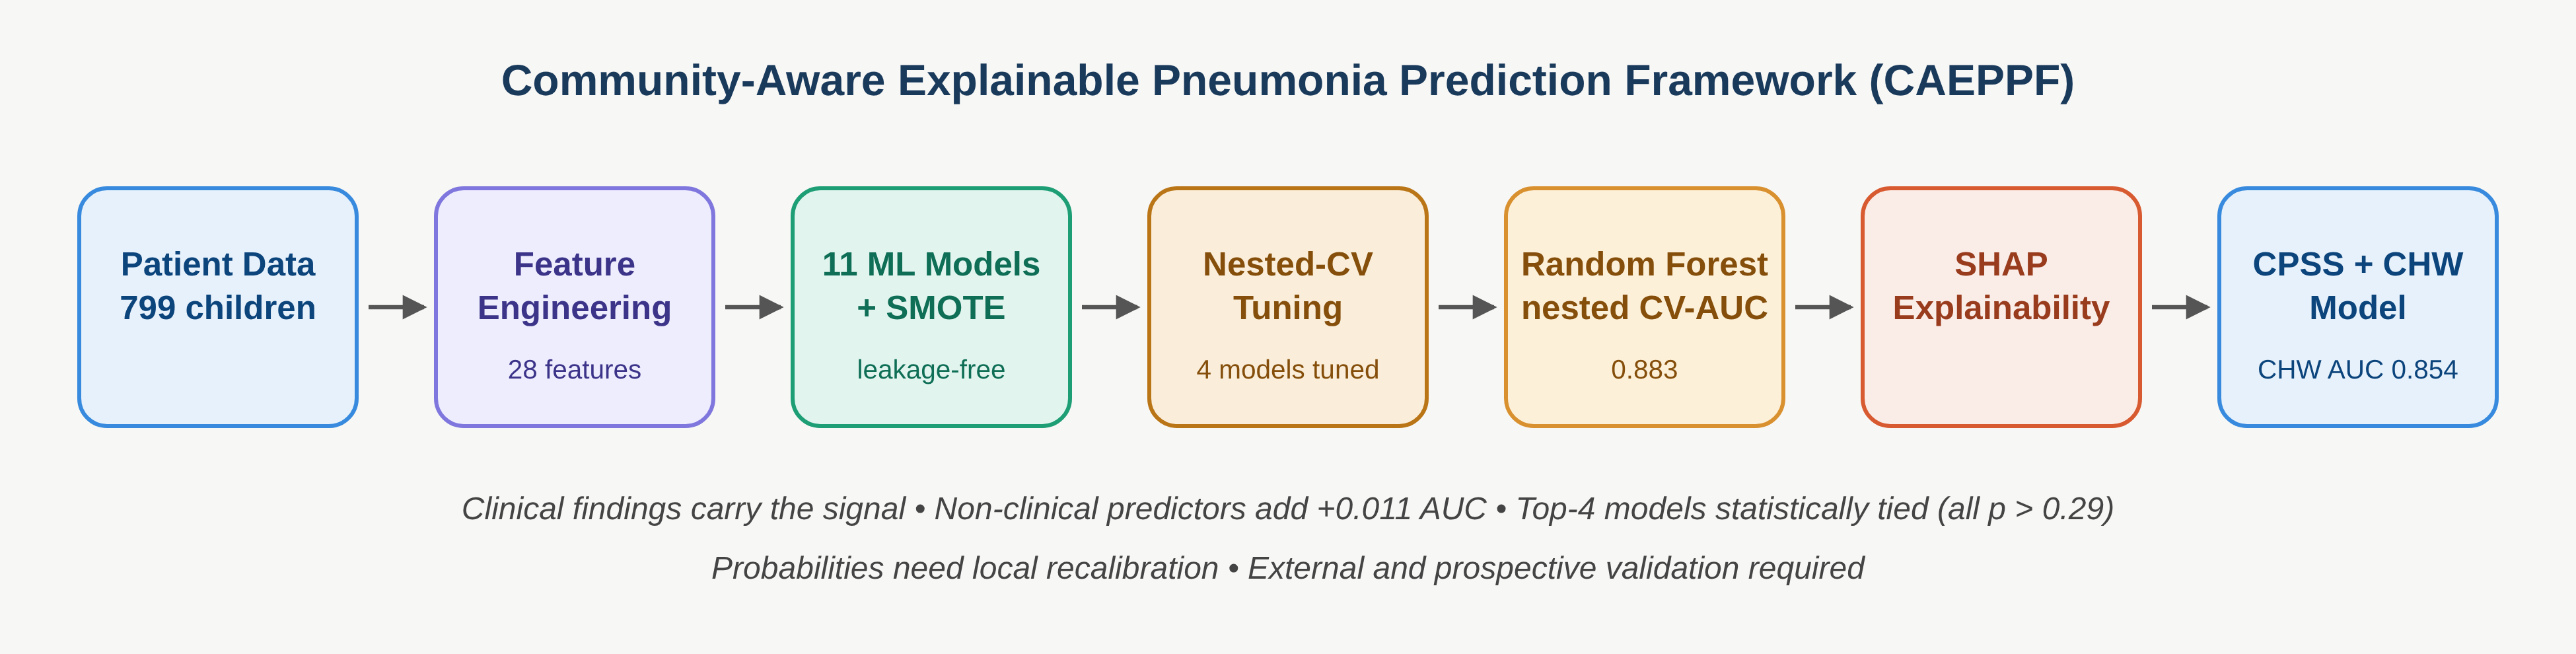
\includegraphics[width=\textwidth]{graphical_abstract.png}
\end{graphicalabstract}

\begin{highlights}
\item Eleven classifiers compared with nested CV; all settings and ranges reported
\item Random Forest selected (nested CV-AUC 0.883); top four models statistically tied
\item Socio-environmental variables alone added no discriminative information
\item Vaccination showed the clearest community-level gradient; crowding did not
\item 22-predictor CHW model reached test AUC 0.854; five-item score reached 0.847
\end{highlights}

%% ===================== ABSTRACT (TRIPOD+AI for Abstracts) =====================
\begin{abstract}
\textbf{Background:} Childhood pneumonia is the leading infectious cause of death in children
under five years, mainly in low- and middle-income countries, where laboratory tests and
radiography are often unavailable at first contact. \textbf{Objectives:} To develop and
internally validate diagnostic multivariable machine learning models for a pneumonia diagnosis
in hospitalized children, and to test whether household crowding, vaccination status and
passive smoking add predictive information. \textbf{Methods:} Data source: a public single-
centre dataset from the Children's Hospital of Rabat, Morocco (children admitted with acute
respiratory infection; 801 records, 799 analysed after excluding two with missing critical
variables). Outcome: a pneumonia-related main admission diagnosis, assessed at presentation (no
follow-up). Eleven classifiers using 28 predictors were compared in a leakage-free pipeline
(imputation, scaling and SMOTE inside every fold); four were tuned by randomized search, and
the final model was chosen by nested 5-fold cross-validation on an 80\% training set (n = 639)
and evaluated once on a 20\% held-out test set (n = 160). Performance was assessed by
discrimination (AUC), calibration, decision-curve net benefit, DeLong and McNemar tests,
subgroup and sensitivity analyses. \textbf{Results:} Of 799 children, 218 (27.3\%) had
pneumonia. Random Forest (28 predictors; wheezing, temperature, procalcitonin and CRP the most
important) was selected: nested CV-AUC 0.883 (95\% CI 0.836--0.931), test AUC 0.881 (95\% CI
0.809--0.938); the four leading models were statistically indistinguishable (all p > 0.29).
Probabilities were over-predicted (mean 0.29--0.34 vs observed 0.275) and needed recalibration.
Socio-environmental variables alone added no discrimination ($-$0.002 CV-AUC); vaccination
showed the clearest gradient (pneumonia 25.2\%, 40.2\%, 57.1\% in fully, partially and un-
vaccinated children). A 22-predictor model without laboratory, radiographic or examination
inputs reached test AUC 0.854 (0.785--0.917) and a five-item score 0.847 (0.771--0.915).
\textbf{Discussion:} Discrimination was good but internal only, from one hospital with a case-
mix of other respiratory diagnoses; external and prospective validation, recalibration and
fairness assessment are needed before any use. \textbf{Registration:} not registered (secondary
analysis of public data).
\end{abstract}

%% ===================== KEYWORDS =====================
\begin{keywords}
Childhood pneumonia \sep Machine learning \sep Feature ablation \sep Community Exposure Risk Score \sep SMOTE \sep SHAP \sep Probability calibration \sep Decision curve analysis \sep DeLong test \sep Fairness analysis \sep Household crowding \sep Vaccination \sep Low- and middle-income countries \sep Community health worker
\end{keywords}

\end{frontmatter}

\section{Introduction}
\label{sec:intro}

Pneumonia is the leading infectious cause of death in children under five years of age worldwide, claiming approximately 700,000 lives annually, with over 95\% of cases concentrated in low- and middle-income countries (LMICs) \cite{r1,r2,r3,r4}. The diagnostic and management gap between high-resource and resource-constrained settings is particularly acute: laboratory biomarkers, chest radiography, and specialist clinical assessment that anchor diagnosis in high-income settings are frequently unavailable to the community health workers (CHWs) and primary care clinicians who serve as the first point of contact for febrile children in LMIC settings \cite{r5,r6}.

Machine learning (ML) has emerged as a powerful approach for structured-data risk prediction, offering the capacity to integrate heterogeneous predictors -- clinical biomarkers, demographic variables, and socio-environmental determinants -- into probabilistic risk estimates that could inform triage decisions in resource-limited settings. However, the ML literature on pediatric pneumonia suffers from four persistent methodological gaps: (1) absence of feature ablation studies quantifying the independent contribution of socio-environmental determinants over clinical baselines; (2) reliance on expert-defined rather than data-optimized composite risk indices; (3) omission of clinical validity assessments including probability calibration and decision curve analysis, increasingly required by medical AI reviewers; and (4) lack of fairness evaluation across demographic subgroups, despite growing recognition of algorithmic bias in clinical prediction models.


\subsection{Socio-environmental determinants of childhood pneumonia}

Household crowding operates as a contact-structure variable increasing pathogen exposure frequency and dose \cite{r3,r7}. Howie et al. demonstrated that bed-sharing with a symptomatic individual was independently associated with elevated pneumonia risk (OR = 2.1, 95\% CI: 1.3--3.4) in The Gambia \cite{r8}. Kamruzzaman et al. identified households with three or more persons per room as significantly higher-risk in Bangladesh \cite{r3}. Vaccination exerts direct and indirect protective effects against vaccine-preventable serotypes; da Fonseca Lima et al. showed unvaccinated children had 2.8$\times$ the odds of community-acquired pneumonia compared to fully immunized peers \cite{r9}. Secondhand tobacco smoke impairs mucociliary defence and predisposes to lower respiratory tract infections \cite{r1,r3,r10}, though binary self-report measurement limits its individual-level discriminatory power \cite{r6,r10}.

\subsection{Existing prediction models and methodological gaps}
\label{sec:litrev}

Image-based diagnostic ML models dominate the pediatric pneumonia literature, with capsule networks (97.2\% accuracy) \cite{r11} and deep residual networks (96.7\%) \cite{r12} addressing a fundamentally different imaging diagnostic task unavailable in LMIC primary care. Among structured-data models, Serin et al. (AUC = 0.87) modeled clinical severity escalation \cite{r4} and Demsash et al. (AUC = 0.91) used nutritional and demographic features \cite{r7}. Neither study conducted feature ablation analysis, proposed a composite socio-environmental index, reported probability calibration or decision curve analysis, performed subgroup fairness evaluation, or developed a deployable clinical scoring system -- gaps that this paper addresses.

\subsection{Clinical validity requirements for medical AI}

Medical AI publications increasingly require evidence of clinical validity beyond discriminative performance. Calibration -- the agreement between predicted probabilities and observed outcomes -- is essential for models whose outputs drive clinical decisions, since a model with AUC = 0.89 but systematic overconfidence may cause inappropriate triage \cite{r13}. Decision curve analysis (DCA) quantifies net clinical benefit across decision thresholds, answering whether a model improves outcomes compared to default clinical strategies \cite{r4}. Fairness analysis evaluates whether predictive performance is equitably distributed across demographic subgroups, addressing a growing concern in clinical AI deployment \cite{r14}. This study addresses all three requirements.

\subsection{Target population, intended use and users}
\label{sec:tpop}
 The target population is children admitted to hospital with an acute respiratory infection, and the outcome is a pneumonia-related diagnosis at presentation. The models are diagnostic rather than prognostic: they estimate the probability that a child's presentation corresponds to pneumonia, to support triage and referral decisions in the care pathway. The intended users are hospital and primary-care clinicians (full 28-predictor model) and community health workers (22-predictor CHW model and five-item points score). At this stage the work is a development and internal-validation study; none of the models is ready for clinical use. Existing ML studies for pediatric pneumonia are reviewed in Section~\ref{sec:litrev} \cite{r4,r7}.

\subsection{Known health inequalities}
\label{sec:ineq}
 The burden of childhood pneumonia is concentrated in low- and middle-income countries and, within them, among children living in crowded households, with incomplete vaccination, exposure to tobacco smoke and limited access to care \cite{r1,r5,r8,r13}. These sociodemographic gradients motivate the socio-environmental predictors and the subgroup analysis by sex, age group and vaccination status (Section~\ref{sec:fairm}).

\subsection{Objectives and contributions}
\label{sec:obj}

This paper addresses these four gaps through the Community-Aware Explainable Pneumonia Prediction Framework (CAEPPF) -- an integrated research framework built on a clinical pediatric dataset of 799 children. The framework is named to reflect its three distinguishing properties: community-awareness (explicit encoding and quantification of household crowding, vaccination, and passive smoking as structured ML features), explainability (SHAP importance, dependence plots, and individual explanations), and prediction (a statistically compared, multi-algorithm benchmark with calibration and decision-curve assessment). To our knowledge, no earlier ML study of pediatric pneumonia has reported feature ablation, CERS weight optimization, probability calibration, decision curve analysis, DeLong/McNemar tests, subgroup analysis, SHAP dependence plots, and sensitivity analysis together. Because the validity of such a comparison depends on how each model was built, this revision describes every algorithm, its parameter settings, the tuning and model-selection procedure, and the full analytic workflow in sufficient detail for independent replication.

The nine principal contributions of CAEPPF are:

\begin{enumerate}[leftmargin=1.6em,itemsep=2pt,topsep=3pt]
\item \textbf{Feature ablation study ($\Delta$AUC):} Five controlled configurations (A--E) quantify the incremental cross-validated AUC contributed by each feature category. All 28 features improved on the clinical-only baseline by +0.011 AUC, whereas adding the socio-environmental variables alone changed it by $-$0.002.
\item \textbf{Data-driven CERS optimization:} Logistic regression coefficients provide empirically estimated CERS weights (Smoking = 0.176, VaccRisk = 0.698, HHSize = 0.126, PersonsPerRoom = 0.000 after truncating a negative coefficient), compared against expert-defined weights on held-out data.
\item \textbf{Transparent 11-algorithm benchmarking:} A leakage-free SMOTE pipeline, explicit reasons for the choice of every algorithm, randomized hyperparameter search (20--40 draws) for four models, nested cross-validation for model selection, and 95\% confidence intervals for all CV-AUC and test-AUC values.
\item \textbf{DeLong and McNemar statistical tests:} Pairwise AUC and prediction-agreement tests across the four leading models, determining whether performance differences are statistically significant.
\item \textbf{Probability calibration:} Calibration curves, Brier scores, and Expected Calibration Error (ECE) for all models, plus Platt recalibration of the two models proposed for use.
\item \textbf{Decision Curve Analysis (DCA):} Net benefit curves for the four leading models compared against treat-all and treat-none strategies.
\item \textbf{Fairness / subgroup analysis:} AUC with bootstrap confidence intervals and recall evaluated across six demographic subgroups (sex, age group, vaccination status).
\item \textbf{Expanded SHAP interpretability:} SHAP summary, dependence plots (top four features), and individual explanations for representative low-, intermediate-, and high-risk patients.
\item \textbf{Sensitivity analysis:} AUC stability across ten random train--test splits (Random Forest: mean = 0.887, SD = 0.021).
\end{enumerate}

The framework additionally evaluates a community-level model restricted to 22 predictors that a CHW could plausibly collect, and points score (CPSS) derived from five easily collected predictors.

\section{Methods}
\label{sec:meth}
This is a study to develop and internally validate diagnostic multivariable prediction models (TRIPOD+AI type 1b: development with internal validation by data splitting and cross-validation). It is reported according to the TRIPOD+AI statement \cite{r34}; the completed checklist, with the section in which each item is reported, is given in Table~\ref{tab:tripod}.

\subsection{Study design and analytic workflow}

The study followed one sequential workflow, summarized in Fig.~\ref{fig:1}. (i) The public dataset was converted into a binary target and 28 predictors (Table~\ref{tab:1}). (ii) Records missing any of four critical variables were excluded; every other gap was imputed inside the modelling pipeline. (iii) The data were split once into a stratified training set (80\%, n = 639) and a test set (20\%, n = 160). (iv) All model development, namely hyperparameter tuning, cross-validated comparison and model selection, used the training set only. (v) The selected model and its competitors were then evaluated once on the test set. (vi) Supporting analyses (feature-group ablation, CERS and CPSS derivation, the community-level model, SHAP, subgroup and sensitivity analyses) used the same split and pipeline. Every data-dependent operation (imputation, scaling, oversampling, hyperparameter search, derivation of CERS weights and CPSS points) was fitted on training data only, so the test set could not influence any modelling decision.

\begin{figure*}[tbp]
\centering
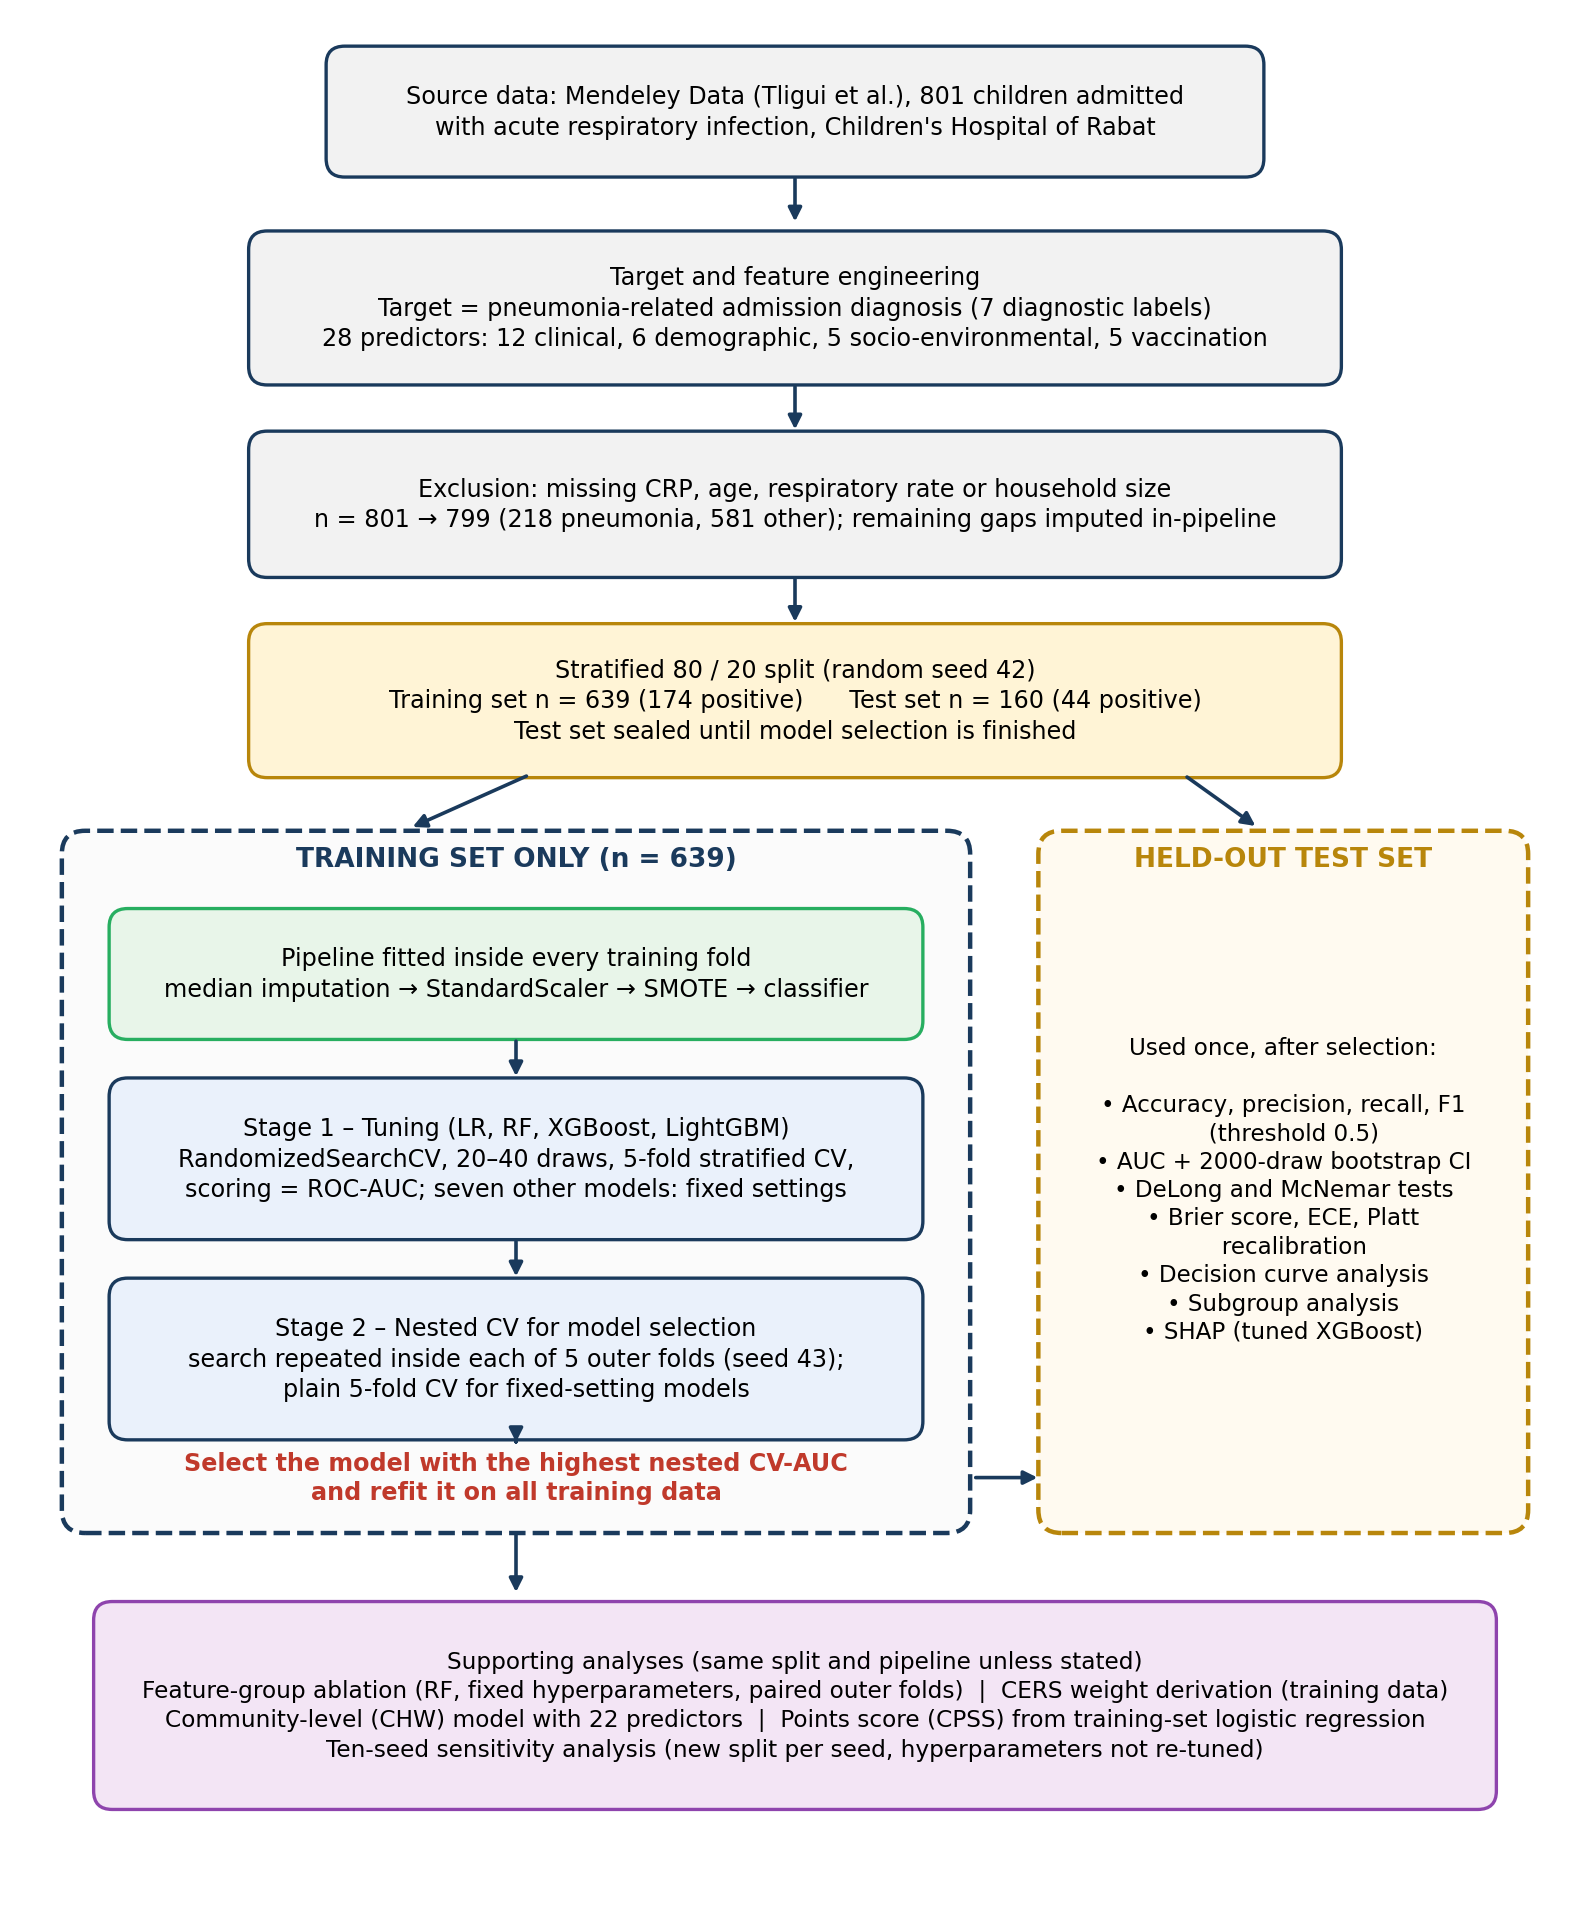
\includegraphics[width=0.60\textwidth]{fig01.png}
\caption{Analytic workflow of CAEPPF, from data source to model selection and held-out evaluation. Dashed boxes separate operations restricted to the training set from those performed once on the test set.}
\label{fig:1}
\end{figure*}

\subsection{Ethics statement}
\label{sec:eth}

This study is a secondary analysis of a publicly available, fully anonymized dataset (Mendeley Data, CC BY 4.0, DOI: 10.17632/2d9dvnycjw.1), originally collected from 801 children admitted to the Children’s Hospital of Rabat, Morocco with acute pediatric respiratory infections \cite{r15}. No patients were recruited, contacted, or followed by the authors as part of this study, and all data were de-identified prior to public release by the original data custodians. Institutional review board (IRB) approval was not required for this secondary analysis of de-identified, publicly available data, in accordance with standard ethical guidelines governing secondary data research. No animal subjects were used in this study.

\subsection{Study setting, participants and study period}
\label{sec:setting}

The data come from a single centre, the Children's Hospital of Rabat, Morocco, a tertiary pediatric hospital (secondary-to-tertiary care setting), and were released as a public dataset \cite{r15}. Participants are children admitted with an acute pediatric respiratory infection; the only additional eligibility requirement we applied was availability of four critical variables (Section~\ref{sec:incl}). The same dataset was used for development and evaluation, through a random stratified split (Section~\ref{sec:part}). The accrual start and end dates are those given by the data custodians \cite{r15} [authors to insert the dates from the data descriptor]; there was no follow-up, because the outcome is the diagnosis recorded at admission. Treatments received were not among the predictors and are not relevant to a diagnostic model applied at presentation.

\subsection{Dataset and target variable}
\label{sec:data}

The dataset was assembled from 801 children admitted to the Children’s Hospital of Rabat, Morocco with acute pediatric respiratory infections by Tligui et al. \cite{r15}. The binary outcome (target = 1, pneumonia-positive) was derived from the recorded main admission diagnosis and set to 1 for any of seven labels: pneumonia, dyspneic pneumopathy, staphylococcal pneumonia, bronchiolitis with pneumonia, asthma attack with pneumonia, pleuropneumonitis, and interstitial pneumopathy. All other main diagnoses (for example, bronchiolitis or asthma without pneumonia) were coded 0. The comparison group is therefore other acute respiratory infections in hospitalized children, not healthy children, and the task is to discriminate a pneumonia diagnosis within this hospitalized population.

\subsection{Inclusion, exclusion and missing data}
\label{sec:incl}

Four variables were treated as critical, namely C-reactive protein (CRP), age, respiratory rate and household size. Records missing any of them were excluded (801 to 799 records; both exclusions lacked household size), leaving 218 positive (27.3\%) and 581 negative (72.7\%) cases. The remaining predictors contained missing values (before exclusion: chest X-ray 62 records, 7.74\%; oxygen saturation 34, 4.24\%; procalcitonin 17, 2.12\%; heart rate 13, 1.62\%; rooms and persons-per-room 4, 0.50\% each; temperature 3, 0.37\%; number of siblings 2, 0.25\%). These were not imputed before splitting. Instead, a median imputer was the first step of the modelling pipeline and was re-fitted on the training portion of each cross-validation fold, so no information from validation or test records entered the imputed values.

\subsection{Sample size}
\label{sec:ss}

The sample size was fixed by the public dataset (799 analysed children, 218 events); no formal sample-size calculation was possible. The training set held 639 children with 174 events, giving about 6.2 events per candidate predictor for the 28-predictor model and 7.9 for the 22-predictor CHW model, which is low for unpenalised regression. We therefore relied on tree ensembles and a regularised logistic baseline, nested cross-validation for model selection, and confidence intervals for every estimate; the test set (160 children, 44 events) was used once and gives wide intervals. The consequences for precision and for subgroup and calibration estimates are discussed in Section~\ref{sec:lim}.

\subsection{Feature engineering (28 predictors)}
\label{sec:feat}

Twenty-eight predictors were constructed across four categories: clinical biomarkers and signs (12), demographic (6), socio-environmental (5) and vaccination (5). Their definitions and encodings are listed in Table~\ref{tab:1}. Persons-per-room was computed as household size divided by number of rooms. Age-appropriate vaccination status was one-hot encoded into three indicators, and the chest X-ray finding was ordinally encoded. No predictor was dropped, transformed (other than scaling), or selected using the outcome (see Feature selection strategy below).

\begin{table*}[tbp]
\caption{Definition and encoding of the 28 predictors.}
\label{tab:1}
\centering
{\scriptsize
\setlength{\tabcolsep}{3.2pt}
\begin{tabular}{>{\raggedright\arraybackslash}p{0.186\textwidth}>{\raggedright\arraybackslash}p{0.249\textwidth}>{\raggedright\arraybackslash}p{0.508\textwidth}}
\toprule
\textbf{Category} & \textbf{Predictor} & \textbf{Definition / encoding} \\
\midrule
Clinical (12) & CRP & C-reactive protein, continuous \\
 & Procalcitonin & Continuous \\
 & SaO$_{2}$ & Oxygen saturation at admission, continuous \\
 & Temperature & Axillary temperature ($^{\circ}$C), continuous \\
 & RespiratoryRate & Breaths per minute, continuous \\
 & HeartRate & Beats per minute, continuous \\
 & Fever & History of fever, binary \\
 & Crackles & Binary \\
 & Wheezing & Binary \\
 & NasalFlaring & Binary \\
 & Cyanosis & Binary \\
 & ChestXray & Ordinal: 0 normal, 1 “NF” (as coded in source), 2 other infiltrates, 3 endpoint pneumonia \\
\midrule
Demographic (6) & Age & Months, continuous \\
 & Gender & 1 = male, 0 = female \\
 & Siblings & Count \\
 & Prematurity & Binary \\
 & Breastfed & Binary \\
 & PriorRespAdm & Prior admission for a respiratory condition, binary \\
\midrule
Socio-environmental (5) & HouseholdSize & Persons living in the house, count \\
 & Rooms & Number of rooms, count \\
 & PersonsPerRoom & HouseholdSize $\div$ Rooms (missing if Rooms = 0) \\
 & SmokersAtHome & Passive-smoke exposure, binary self-report \\
 & VitaminA & Vitamin A supplementation, binary \\
\midrule
Vaccination (5) & \texttt{Vacc\_\allowbreak Full} / \texttt{Vacc\_\allowbreak Partial} / \texttt{Vacc\_\allowbreak None} & One-hot indicators of age-appropriate vaccination (“Yes” / “Partially” / “No”) \\
 & HibDoses & Number of Hib vaccine doses \\
 & PneumoDoses & Number of pneumococcal vaccine doses \\
\bottomrule
\end{tabular}}
\end{table*}

\subsection{Data partitioning and prevention of information leakage}
\label{sec:part}

A single stratified 80/20 split (random seed 42) produced a training set of 639 patients (174 positive, 465 negative) and a test set of 160 patients (44 positive, 116 negative). The test set was not used for tuning, model selection, imputation, scaling, oversampling, CERS weight estimation or CPSS point derivation. Model selection used cross-validation on the training set only; the test set was evaluated once for each model after that choice was fixed.

\subsection{Preprocessing and handling of class imbalance}
\label{sec:prep}

Every model was embedded in an identical imbalanced-learn pipeline: (1) median imputation, (2) StandardScaler (zero mean, unit variance), (3) SMOTE \cite{r17} (five nearest neighbours, minority class oversampled to parity, \texttt{random\_\allowbreak state} = 42) and (4) the classifier. Because the imputer, scaler and SMOTE are pipeline steps, they are re-fitted on the training portion of each cross-validation fold; synthetic samples are generated only from training-fold observations, and validation folds and the test set are never resampled. Scaling was applied to tree-based models as well so that all eleven algorithms share one preprocessing path; this does not alter tree splits. SMOTE was chosen because the positive class is a minority (27.3\%) and recall at a fixed threshold is clinically important. It is known to inflate predicted probabilities \cite{r30}, so calibration was assessed explicitly (see below). Alternative imbalance strategies, such as class weighting or no resampling, were not compared.

\subsection{Feature selection strategy}
\label{sec:fsel}

No data-driven feature selection was performed, and all 28 predictors entered every model. This was deliberate. The candidate set is small and was fixed a priori from clinical and epidemiological considerations; the training set contains 174 events, giving roughly six events per candidate predictor, which is limited but acceptable for regularized and ensemble learners; tree ensembles and L2-penalized logistic regression tolerate correlated inputs (for example the three vaccination indicators, which sum to one, and persons-per-room, which is derived from household size and rooms); and selecting features within cross-validation would add a further layer of optimism to be controlled. The contribution of predictor groups was instead examined explicitly through the ablation study, and the importance of individual predictors through random-forest impurity importance and SHAP, both of which are reported but were not used to remove variables.

\subsection{Rationale for the choice of algorithms}
\label{sec:alg}

Eleven supervised classifiers were benchmarked. They were selected against six criteria: (i) coverage of the main families of learners for structured data (linear, single-tree, bagged-tree, boosted-tree, kernel, instance-based, probabilistic and neural), so that conclusions are not specific to one inductive bias; (ii) prior use in pediatric pneumonia and clinical tabular prediction, notably random forest \cite{r4} and gradient-boosted trees \cite{r7}; (iii) suitability for a small dataset (n = 799) with 28 mixed binary, ordinal and continuous predictors; (iv) native probability outputs, which calibration and decision-curve analysis require; (v) interpretability and deployability, since logistic regression coefficients can be turned into a paper-based points score and tree ensembles support exact SHAP attribution \cite{r24}; and (vi) availability in open-source libraries (scikit-learn \cite{r23}, XGBoost \cite{r19}, LightGBM \cite{r20}) so that every model can be reproduced. The reason for including each algorithm, and its configuration, is given in Table~\ref{tab:2}.

Logistic regression was the transparent linear baseline and the only model that can be converted directly into a bedside score. Random forest \cite{r18} was included as the standard bagged ensemble that is robust to noise and small samples. Four boosted-tree learners (gradient boosting, AdaBoost \cite{r31}, XGBoost, LightGBM) were included because gradient-boosted trees are the most consistently strong family on medium-sized tabular data \cite{r25}; they differ in loss, tree growth and regularization and therefore test whether any one implementation is superior. The decision tree gives a fully readable but high-variance reference. The RBF support vector machine \cite{r32}, k-nearest neighbours, Gaussian naive Bayes and multilayer perceptron stand for kernel, instance-based, probabilistic and neural approaches; they establish whether a fundamentally different decision-boundary assumption would outperform tree and linear models on these data.

Several well-known approaches were intentionally not included. Convolutional and residual networks, and vision transformers, require images and address a different diagnostic task \cite{r11,r12}. Deep tabular architectures (for example TabNet or FT-Transformer) typically need much larger samples and extensive tuning, and tree-based models usually match or exceed them on datasets of this size \cite{r25}. CatBoost is a further gradient-boosted tree implementation and would add little diversity beyond the four boosting methods already included. Linear and quadratic discriminant analysis share the linear boundary of logistic regression but add distributional assumptions that binary predictors violate. Penalized logistic regression with sparsity (lasso or elastic net) was not used because feature selection was not a goal; the L2 strength was tuned instead. Generalized additive and explainable boosting models are interesting interpretable alternatives and are noted as future work. Voting or stacking ensembles were not evaluated, because the four leading single models were statistically indistinguishable (see Results) and there was no basis for expecting a gain from combining them in n = 799.

\begin{table*}[tbp]
\caption{The eleven algorithms: family, reason for inclusion, and configuration. All were run inside the same preprocessing pipeline; \texttt{random\_\allowbreak state} = 42 where applicable. Unlisted parameters are scikit-learn 1.6.1 defaults.}
\label{tab:2}
\centering
{\scriptsize
\setlength{\tabcolsep}{3.2pt}
\begin{tabular}{>{\raggedright\arraybackslash}p{0.144\textwidth}>{\raggedright\arraybackslash}p{0.118\textwidth}>{\raggedright\arraybackslash}p{0.365\textwidth}>{\raggedright\arraybackslash}p{0.303\textwidth}}
\toprule
\textbf{Algorithm} & \textbf{Family} & \textbf{Reason for inclusion} & \textbf{Configuration} \\
\midrule
Logistic regression & Linear, parametric & Interpretable baseline; coefficients convertible to a points score; best-practice reference for clinical risk models & Tuned: L2 penalty; C, solver, \texttt{max\_\allowbreak iter} searched (Table~\ref{tab:3}) \\
Decision tree & Single tree & Fully readable rules; shows the gain from ensembling & \texttt{max\_\allowbreak depth} = 5, \texttt{min\_\allowbreak samples\_\allowbreak split} = 10 \\
Random forest & Bagged trees & Robust to noise and small n; handles non-linearity and interactions; impurity importance & Tuned: \texttt{n\_\allowbreak estimators}, \texttt{max\_\allowbreak depth}, \texttt{min\_\allowbreak samples\_\allowbreak split}, \texttt{min\_\allowbreak samples\_\allowbreak leaf}, \texttt{max\_\allowbreak features} \\
Gradient boosting (scikit-learn) & Boosted trees & Classical boosting reference for the modern implementations & \texttt{n\_\allowbreak estimators} = 200, \texttt{learning\_\allowbreak rate} = 0.1, \texttt{max\_\allowbreak depth} = 3 (default) \\
AdaBoost & Boosted stumps & Adaptive re-weighting boosting; different loss from gradient boosting & \texttt{n\_\allowbreak estimators} = 100, \texttt{learning\_\allowbreak rate} = 1.0 (default), depth-1 trees \\
XGBoost & Regularized boosted trees & Widely used on tabular clinical data \cite{r7}; exact TreeSHAP; strong regularization & Tuned: \texttt{n\_\allowbreak estimators}, \texttt{max\_\allowbreak depth}, \texttt{learning\_\allowbreak rate}, subsample, \texttt{colsample\_\allowbreak bytree} \\
LightGBM & Leaf-wise boosted trees & Efficient boosting with a different tree-growth strategy & Tuned: \texttt{n\_\allowbreak estimators}, \texttt{num\_\allowbreak leaves}, \texttt{learning\_\allowbreak rate}, subsample, \texttt{colsample\_\allowbreak bytree}, \texttt{min\_\allowbreak child\_\allowbreak samples} \\
SVM (RBF) & Kernel method & Non-linear margin classifier; tests a non-tree, non-linear boundary & C = 1.0, gamma = “scale”, probability = True \\
k-nearest neighbours & Instance-based & Local, assumption-free reference & k = 7 (odd, avoids ties), Euclidean distance, uniform weights \\
Gaussian naive Bayes & Probabilistic & Fast generative baseline; tests independence assumption & Defaults (\texttt{var\_\allowbreak smoothing} = 1e-9) \\
MLP & Neural network & Small feed-forward network; tests whether a neural model helps at n = 799 & Two hidden layers (100, 50), ReLU, Adam, \texttt{max\_\allowbreak iter} = 500, alpha = 1e-4 (default) \\
\bottomrule
\end{tabular}}
\end{table*}

\subsection{Hyperparameter tuning and parameter settings}
\label{sec:hyp}

Four models were tuned: logistic regression, random forest, XGBoost and LightGBM. They were chosen a priori to represent the linear, bagged-tree and boosted-tree families, and the three non-linear models are the most flexible learners and so the most sensitive to hyperparameters. Random forest was added to the tuned set to ensure a fair comparison with the strongest baseline learner. The remaining seven models were run with the fixed, conventional settings in Table~\ref{tab:2} to bound computation, because nested tuning of all eleven models multiplies run time several-fold; the consequences of this decision are discussed under Limitations.

Tuning used scikit-learn RandomizedSearchCV on the training set, applied to the full pipeline so that imputation, scaling and SMOTE were re-fitted within each of the five stratified folds (shuffled, random seed 42). The objective was ROC-AUC. Random search was preferred to grid search because it explores continuous and integer parameters more efficiently when only a few parameters matter \cite{r21}. Forty parameter combinations were drawn for random forest, XGBoost and LightGBM, and 20 for logistic regression (three parameters). Each search refitted the best combination on all training data (refit = True, scikit-learn default). The search ranges and the selected values are in Table~\ref{tab:3}. Parameters not listed were fixed at library defaults, with \texttt{random\_\allowbreak state} = 42 (XGBoost additionally \texttt{eval\_\allowbreak metric} = “logloss”).

\begin{table*}[tbp]
\caption{Hyperparameter search spaces and final selected values (5-fold stratified CV, objective ROC-AUC, seed 42).}
\label{tab:3}
\centering
{\scriptsize
\setlength{\tabcolsep}{3.2pt}
\begin{tabular}{>{\raggedright\arraybackslash}p{0.249\textwidth}>{\raggedright\arraybackslash}p{0.228\textwidth}>{\raggedright\arraybackslash}p{0.270\textwidth}>{\raggedright\arraybackslash}p{0.182\textwidth}}
\toprule
\textbf{Model (search budget)} & \textbf{Parameter} & \textbf{Search space} & \textbf{Selected value} \\
\midrule
Logistic regression (20 draws) & C (inverse L2 strength) & Uniform [0.01, 10.01] & 0.216 \\
 & solver & \{lbfgs, saga\} & saga \\
 & \texttt{max\_\allowbreak iter} & \{500, 1000\} & 1000 \\
\midrule
Random forest (40 draws) & \texttt{n\_\allowbreak estimators} & Integer 100--400 & 161 \\
 & \texttt{max\_\allowbreak depth} & \{None, 5, 8, 10, 12, 15\} & 10 \\
 & \texttt{min\_\allowbreak samples\_\allowbreak split} & Integer 2--10 & 8 \\
 & \texttt{min\_\allowbreak samples\_\allowbreak leaf} & Integer 1--5 & 1 \\
 & \texttt{max\_\allowbreak features} & \{sqrt, log2, None\} & log2 \\
\midrule
XGBoost (40 draws) & \texttt{n\_\allowbreak estimators} & Integer 100--399 & 151 \\
 & \texttt{max\_\allowbreak depth} & Integer 3--7 & 3 \\
 & \texttt{learning\_\allowbreak rate} & Uniform [0.01, 0.21] & 0.0316 \\
 & subsample & Uniform [0.6, 1.0] & 0.825 \\
 & \texttt{colsample\_\allowbreak bytree} & Uniform [0.6, 1.0] & 0.610 \\
\midrule
LightGBM (40 draws) & \texttt{n\_\allowbreak estimators} & Integer 100--399 & 199 \\
 & \texttt{num\_\allowbreak leaves} & Integer 20--79 & 59 \\
 & \texttt{learning\_\allowbreak rate} & Uniform [0.01, 0.21] & 0.0216 \\
 & subsample* & Uniform [0.6, 1.0] & 0.883 \\
 & \texttt{colsample\_\allowbreak bytree} & Uniform [0.6, 1.0] & 0.662 \\
 & \texttt{min\_\allowbreak child\_\allowbreak samples} & Integer 5--29 & 28 \\
\bottomrule
\end{tabular}}
\par\smallskip{\scriptsize\raggedright $^{*}$LightGBM applies row subsampling only when \texttt{subsample\_\allowbreak freq} > 0; because \texttt{subsample\_\allowbreak freq} was left at its default of 0, this parameter had no effect on the fitted model}
\end{table*}

\subsection{Model selection and cross-validated validation}
\label{sec:sel}

The primary selection criterion was the mean cross-validated ROC-AUC on the training set. For the four tuned models this was a nested estimate: the complete search was re-run inside each of five outer folds (stratified, shuffled, random seed 43, distinct from the tuning folds), so the outer-fold AUC is not biased by the choice of hyperparameters on the same data \cite{r22}. For the seven fixed-setting models there is no search to nest, and the same outer folds were used with plain cross-validation. For comparison, the optimistic tuning-CV AUC (best inner score) is also reported. Five folds were chosen because each validation fold then contains about 128 patients and 35 events, whereas ten folds would leave about 17 events per fold, making fold-level AUC unstable. The cross-validation interval is the t-based 95\% CI of the mean of the five fold AUCs; because the folds share training data, it is approximate and probably somewhat too narrow. The model with the highest nested CV-AUC was selected before any test-set result was computed. Secondary considerations (calibration, interpretability, feasibility at community level) are reported but did not alter the selection.

\subsection{Performance evaluation}
\label{sec:perf}

Each model was refitted on the entire training set and applied once to the test set. Accuracy, precision, recall (sensitivity), F1 and ROC-AUC were computed at the default probability threshold of 0.5; no threshold was tuned. A 95\% confidence interval for test AUC was obtained by stratified percentile bootstrap (2,000 resamples within each class). Confusion matrices were produced for the three models with the highest CV-AUC.

\subsection{Statistical comparison of models}
\label{sec:stat}

Pairwise AUC comparisons among the four leading models used the paired DeLong test, implemented with the fast algorithm of Sun and Xu \cite{r26} (the implementation was verified to reproduce scikit-learn AUCs exactly). Prediction agreement at threshold 0.5 was compared with McNemar’s test \cite{r33} on paired correct/incorrect classifications, using the exact binomial form when discordant pairs numbered fewer than 25 (all comparisons here). Significance was set at $\alpha$ = 0.05; no adjustment was made for the six comparisons, which favours detecting differences and therefore does not weaken the conclusion of no difference.

\subsection{Probability calibration}
\label{sec:calm}

Calibration was assessed on the test set using calibration curves (10 equal-width bins), the Brier score, and expected calibration error (ECE), the bin-size-weighted mean absolute difference between observed event rate and mean predicted probability \cite{r28}. Because SMOTE changes the apparent class prevalence, Platt (sigmoid) recalibration \cite{r29} was additionally fitted to the two models proposed for use (Random Forest and logistic regression) using internal five-fold cross-validation on the training set only, and re-evaluated on the test set.

\subsection{Decision curve analysis}
\label{sec:dcam}

Net benefit was computed on the test set for threshold probabilities from 0.01 to 0.99 in steps of 0.01 as:
\begin{equation}
\mathrm{Net\ Benefit}=\frac{TP}{n}-\frac{FP}{n}\left[\frac{p_t}{1-p_t}\right]
\label{eq:1}
\end{equation}

where $p_t$ is the threshold probability at which referral is considered warranted \cite{r27}. Model curves were compared with the treat-all strategy (using the test-set prevalence of 27.5\%) and the treat-none strategy (net benefit 0). Raw, uncalibrated model probabilities were used.

\subsection{Feature-group ablation study}

Five predictor sets were compared: (A) clinical only (12 predictors); (B) clinical + demographic (18); (C) clinical + socio-environmental (17); (D) clinical + vaccination (17); and (E) all 28 predictors. Each configuration was evaluated with the tuned Random Forest pipeline using the same five outer folds (seed 43) on training data, so that differences between configurations are paired by fold. Hyperparameters were fixed at the values tuned on all 28 predictors (Table~\ref{tab:3}) and were not re-tuned per set. This makes the comparison controlled, but it may slightly favour the full set, which is the one on which the settings were tuned. The incremental effect is reported as the mean paired difference in fold AUC relative to configuration A, with its fold-to-fold standard deviation. Only Random Forest, the selected model, was used for the ablation.

\subsection{Community Exposure Risk Score (CERS)}

CERS combines four community-level variables: persons-per-room (PPR), smokers at home (Smk), vaccination risk (VR; 0 = fully vaccinated, 0.5 = partially, 1 = unvaccinated) and household size (HHS). Variables were median-imputed and min--max scaled to [0, 1] using training-set limits; test values were scaled with the same limits and clipped to [0, 1]. The expert score used fixed, epidemiologically motivated weights (Eq.~\ref{eq:2}). Data-driven weights were obtained by fitting an L2-regularized logistic regression (C = 1) to the four scaled variables on the training set, truncating negative coefficients to zero, and normalizing the remainder to sum to 1 (Eq.~\ref{eq:3}). Raw coefficients are reported so that any truncation is visible. Both scores were evaluated by AUC on the training and test sets.
\begin{equation}
\mathrm{Expert\ CERS}=0.35\,\mathrm{PPR}+0.30\,\mathrm{Smk}+0.20\,\mathrm{VR}+0.15\,\mathrm{HHS}
\label{eq:2}
\end{equation}
\begin{equation}
\mathrm{Optimized\ CERS}=\sum_j w_j x_j,\qquad w_j=\frac{\max(\beta_j,0)}{\sum_k \max(\beta_k,0)}
\label{eq:3}
\end{equation}

\subsection{Community-level (CHW) model and points score (CPSS)}
\label{sec:chwm}

To approximate what a community health worker can collect, a community-level model was fitted using 22 of the 28 predictors, excluding CRP, procalcitonin, oxygen saturation, heart rate, crackles (auscultation) and chest X-ray. The retained predictors were age, sex, siblings, prematurity, breastfeeding, prior respiratory admission, temperature, respiratory rate, fever, wheezing, nasal flaring, cyanosis, all five socio-environmental variables and all five vaccination variables. This list reflects the authors’ judgement and was not validated with CHWs. Random Forest and logistic regression were refitted with their tuned settings on this reduced set; CV-AUC (outer folds) and test AUC were compared with the full model.

The Community Pneumonia Screening Score (CPSS) was derived from a nearly unpenalized logistic regression (C = 10$^{6}$) fitted on the training set to five predictors: wheezing, fever, crowding (persons-per-room $\geq$ 3; this cut-off is an assumption based on prior literature \cite{r3} and was not tuned), vaccination risk (0, 0.5, 1) and smoking. Each coefficient was divided by the largest absolute coefficient, multiplied by 5 and rounded to the nearest 0.5 to give simple points; the score is the sum of points for a child. Risk bands were not pre-specified. They were described afterwards from the observed pneumonia rate by score in the training and test sets, and are therefore descriptive only. The fixed weights proposed in an earlier version of this work (2, 1.5, 1, 1, 0.5) were evaluated for comparison.

\subsection{Model interpretability (SHAP)}

SHAP values \cite{r24} were computed with TreeExplainer for the tuned XGBoost model fitted on the training set, using test-set observations transformed by the fitted imputer and scaler (SHAP values are in log-odds). XGBoost was used because exact TreeSHAP is available and it had the highest test AUC; this means the explanations describe XGBoost, not the selected Random Forest, whose own interpretability is summarized by Gini importance (161 trees, depth 10). Outputs were a summary plot, dependence plots for the four predictors with the largest mean absolute SHAP value, and individual explanations for the test patients with the lowest, closest-to-0.5 and highest predicted probability. A numerical table of mean SHAP values for high versus low predictor values was produced so that every directional statement in the text can be checked.

\subsection{Fairness and subgroup analysis}
\label{sec:fairm}

Using the selected model on the test set, AUC (with 2,000-resample bootstrap CI) and recall at threshold 0.5 were computed for six subgroups: male and female; infants ($\leq$ 12 months) and older children (> 12 months); and fully versus not fully vaccinated (partially or un-vaccinated). Subgroups with fewer than 10 positive cases are flagged as exploratory. No formal test of between-group difference was performed, and the analysis describes performance variation rather than establishing equity.

\subsection{Sensitivity analysis}

To assess dependence on one random split, the already tuned Random Forest and XGBoost pipelines were refitted on a fresh stratified 80/20 split for each of ten seeds (0, 7, 13, 21, 42, 99, 123, 200, 303, 512), with the seed also applied to SMOTE and the classifier. Hyperparameters were held fixed at the values in Table~\ref{tab:3} and were not re-tuned. Because those values were chosen on the seed-42 training set, test sets from other seeds contain some records seen during tuning, so this analysis tests sensitivity to the split but is mildly optimistic as an estimate of external performance.

\subsection{Descriptive statistics}

For context, continuous predictors were compared between outcome groups with the Mann--Whitney U test and categorical predictors with the chi-square test (persons-per-room by quartile). These tests are descriptive, were performed on all 799 eligible records, and were not used to select variables.

\subsection{Model output, classification threshold and model specification}
\label{sec:output}

Each model outputs a predicted probability of a pneumonia-related diagnosis. A hard classification (accuracy, precision, recall, F1, confusion matrices) used the conventional probability threshold of 0.5; the threshold was not tuned, because the clinically appropriate threshold depends on the cost of missed cases against unnecessary referrals, which is examined through net benefit over a range of thresholds (Section~\ref{sec:dcam}). Because SMOTE inflates predicted risks, probabilities must be recalibrated (Platt scaling, Section~\ref{sec:calm}) before being read as absolute risks. The full specification of the selected Random Forest (pipeline steps, tuned and fixed hyperparameters, random seeds) is in Table~\ref{tab:2} and in the run log, and the notebook that refits the model and produces predictions for new records is provided as Supporting Information (S1 File).

\subsection{Training versus evaluation data and clustering}
\label{sec:trev}

Development (training) and evaluation (test) data come from the same hospital, population, eligibility rules, outcome definition and predictor set and differ only by random stratified allocation (80\%/20\%); the evaluation is therefore internal, and no differences in setting, eligibility, outcome or predictors needed to be described. Because there is a single centre, heterogeneity across clusters (hospitals or countries) could not be examined.

\subsection{Software and reproducibility}
\label{sec:soft}

All analyses were run in a single Python notebook (Python 3.13, NumPy 2.1.3, pandas 2.2.3, SciPy 1.16.3, scikit-learn 1.6.1 \cite{r23}, imbalanced-learn 0.14.2, XGBoost 3.4.1, LightGBM 4.6.0, SHAP 0.52.0). A global random seed of 42 governs the split, tuning folds, SMOTE and all classifiers; seed 43 governs the outer folds. Every table and figure in this paper is written by the notebook directly from the run (nothing is typed in by hand), and library versions, selected hyperparameters, split counts and the bootstrap setting are saved to a run log. The notebook, result tables and figures are provided as Supporting Information (S1 File). The dataset is publicly available at the DOI above.

\section{Open science and patient and public involvement}
\label{sec:open}

\subsection{Funding and conflicts of interest}

[Authors to state the funding source and the role of the funder; if none, state that no specific funding was received.] The authors declare no competing interests (see the Declaration of competing interest).

\subsection{Protocol and registration}

No study protocol was prepared and the study was not registered, because it is a secondary analysis of a public dataset.

\subsection{Data and code sharing}

The dataset analyzed is publicly available via Mendeley Data (DOI: 10.17632/2d9dvnycjw.1) under a CC BY 4.0 license \cite{r15}. The analysis notebook (\texttt{Pneumonia\_\allowbreak ML\_\allowbreak Pipeline}.ipynb), which contains the analytical code (data cleaning, feature engineering, model building and evaluation), all result tables (CSV), figures and the run log with library versions and selected hyperparameters are provided as Supporting Information (S1 File).

\subsection{Patient and public involvement}

There was no patient or public involvement in the design, conduct, reporting or interpretation of the study.

\section{Results}
\label{sec:res}

\subsection{Cohort and univariable associations}
\label{sec:cohort}

The analytic cohort comprised 799 children, of whom 218 (27.3\%) had a pneumonia-related diagnosis. Among univariable associations (Mann--Whitney or chi-square), wheezing showed by far the strongest relationship with outcome ($\chi$$^{2}$ = 226.7, p < 0.001), followed by procalcitonin (p < 0.001), temperature (p < 0.001), CRP (p < 0.001), fever ($\chi$$^{2}$ = 54.4, p < 0.001) and crackles ($\chi$$^{2}$ = 35.4, p < 0.001). Among community-level variables, full vaccination was associated with outcome ($\chi$$^{2}$ = 11.1, p < 0.001), whereas passive smoking ($\chi$$^{2}$ = 2.67, p = 0.102) and crowding by quartile of persons-per-room ($\chi$$^{2}$ = 4.81, p = 0.187) were not. Wheezing was inversely related to a pneumonia label: children with wheezing were more likely to carry a diagnosis such as bronchiolitis or asthma, which defines the comparison group in this hospital cohort.

\subsection{Model performance comparison}
\label{sec:mperf}

Table~\ref{tab:4} presents performance for all 11 algorithms, ranked by cross-validated AUC; Fig.~\ref{fig:2} shows the test-set ROC curves, Fig.~\ref{fig:3} the cross-validated AUC with confidence intervals, and Fig.~\ref{fig:4} the confusion matrices of the top three models. Random Forest had the highest nested CV-AUC (0.883, 95\% CI 0.836--0.931) and was therefore selected under the prespecified criterion. Logistic regression (0.877), XGBoost (0.874) and LightGBM (0.869) followed within 0.014 AUC, with heavily overlapping intervals. On the test set the selected Random Forest reached AUC 0.881 (95\% bootstrap CI 0.809--0.938), identical to logistic regression, while XGBoost had the numerically highest test AUC (0.888); this ordering difference is within sampling noise (44 positive test cases) and shows why selection was made on cross-validation and not on the test set.

\begin{figure}[tbp]
\centering
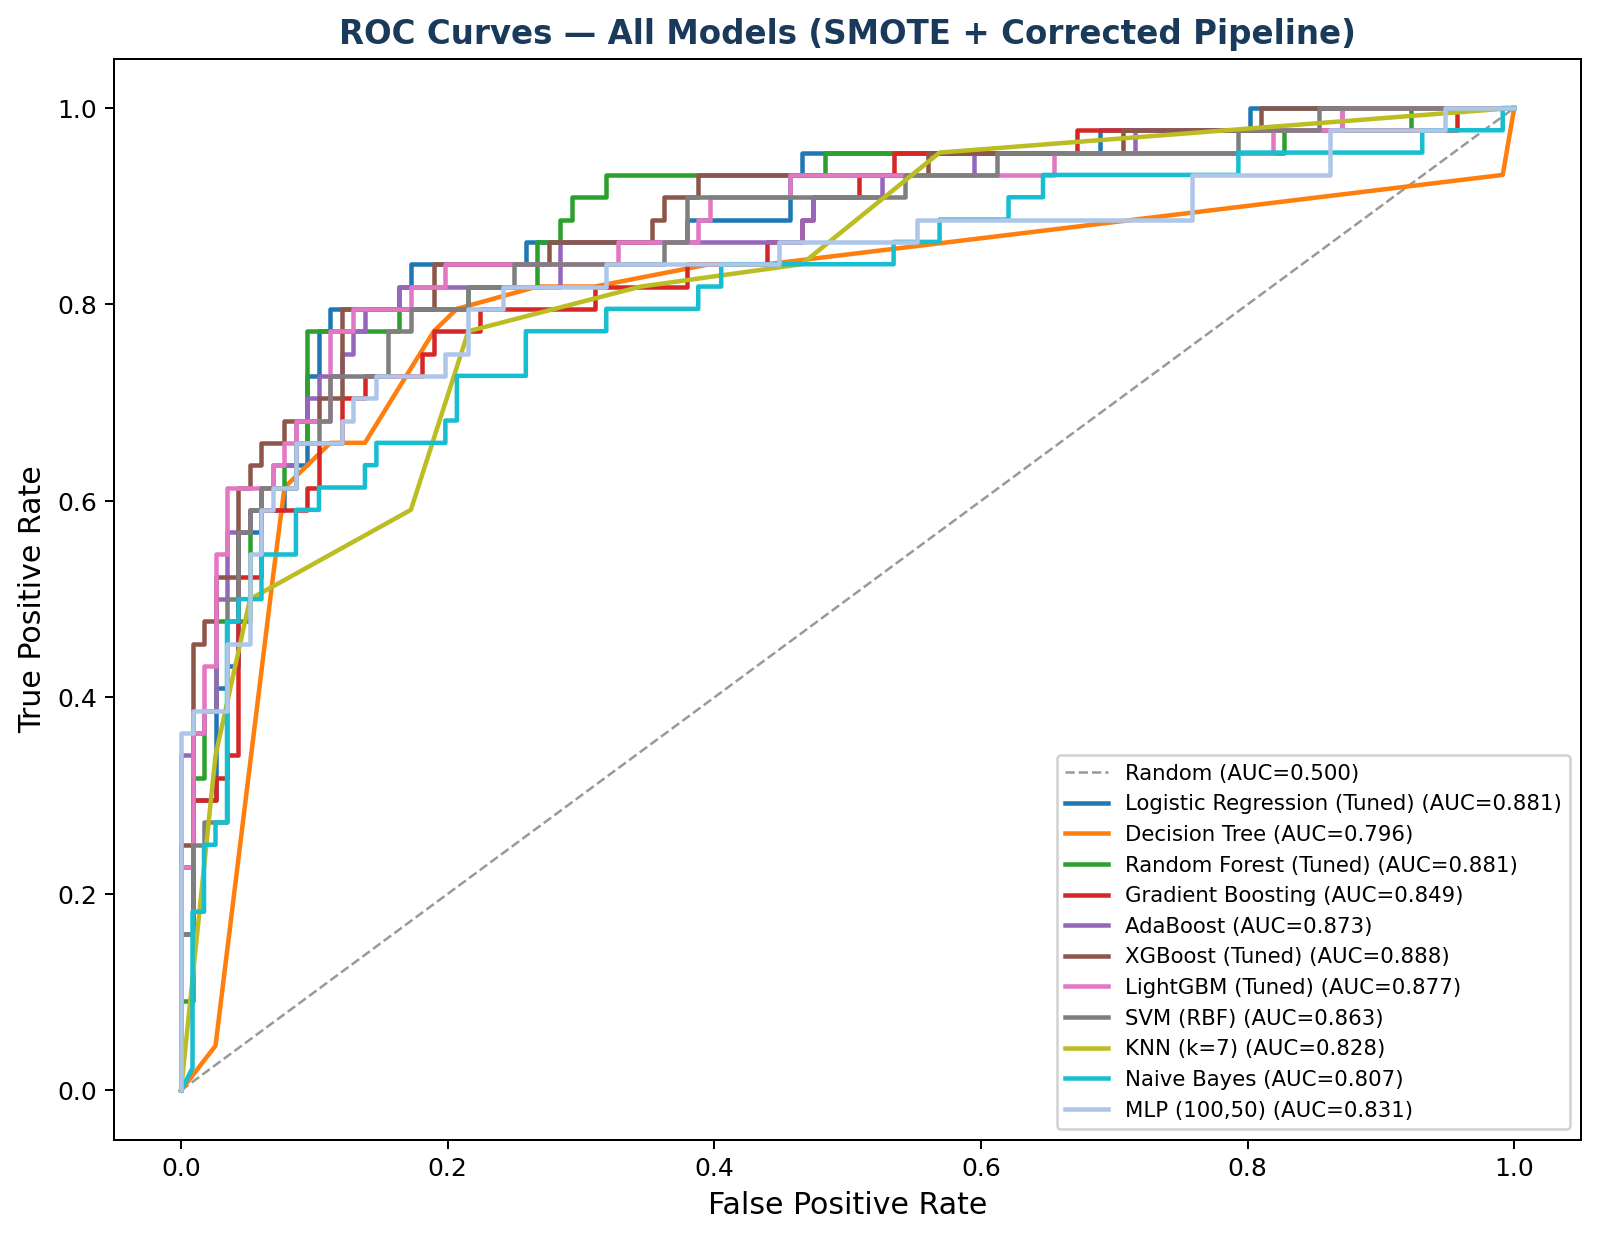
\includegraphics[width=\columnwidth]{fig02.png}
\caption{ROC curves for all 11 models on the held-out test set (n = 160).}
\label{fig:2}
\end{figure}

\begin{figure*}[tbp]
\centering
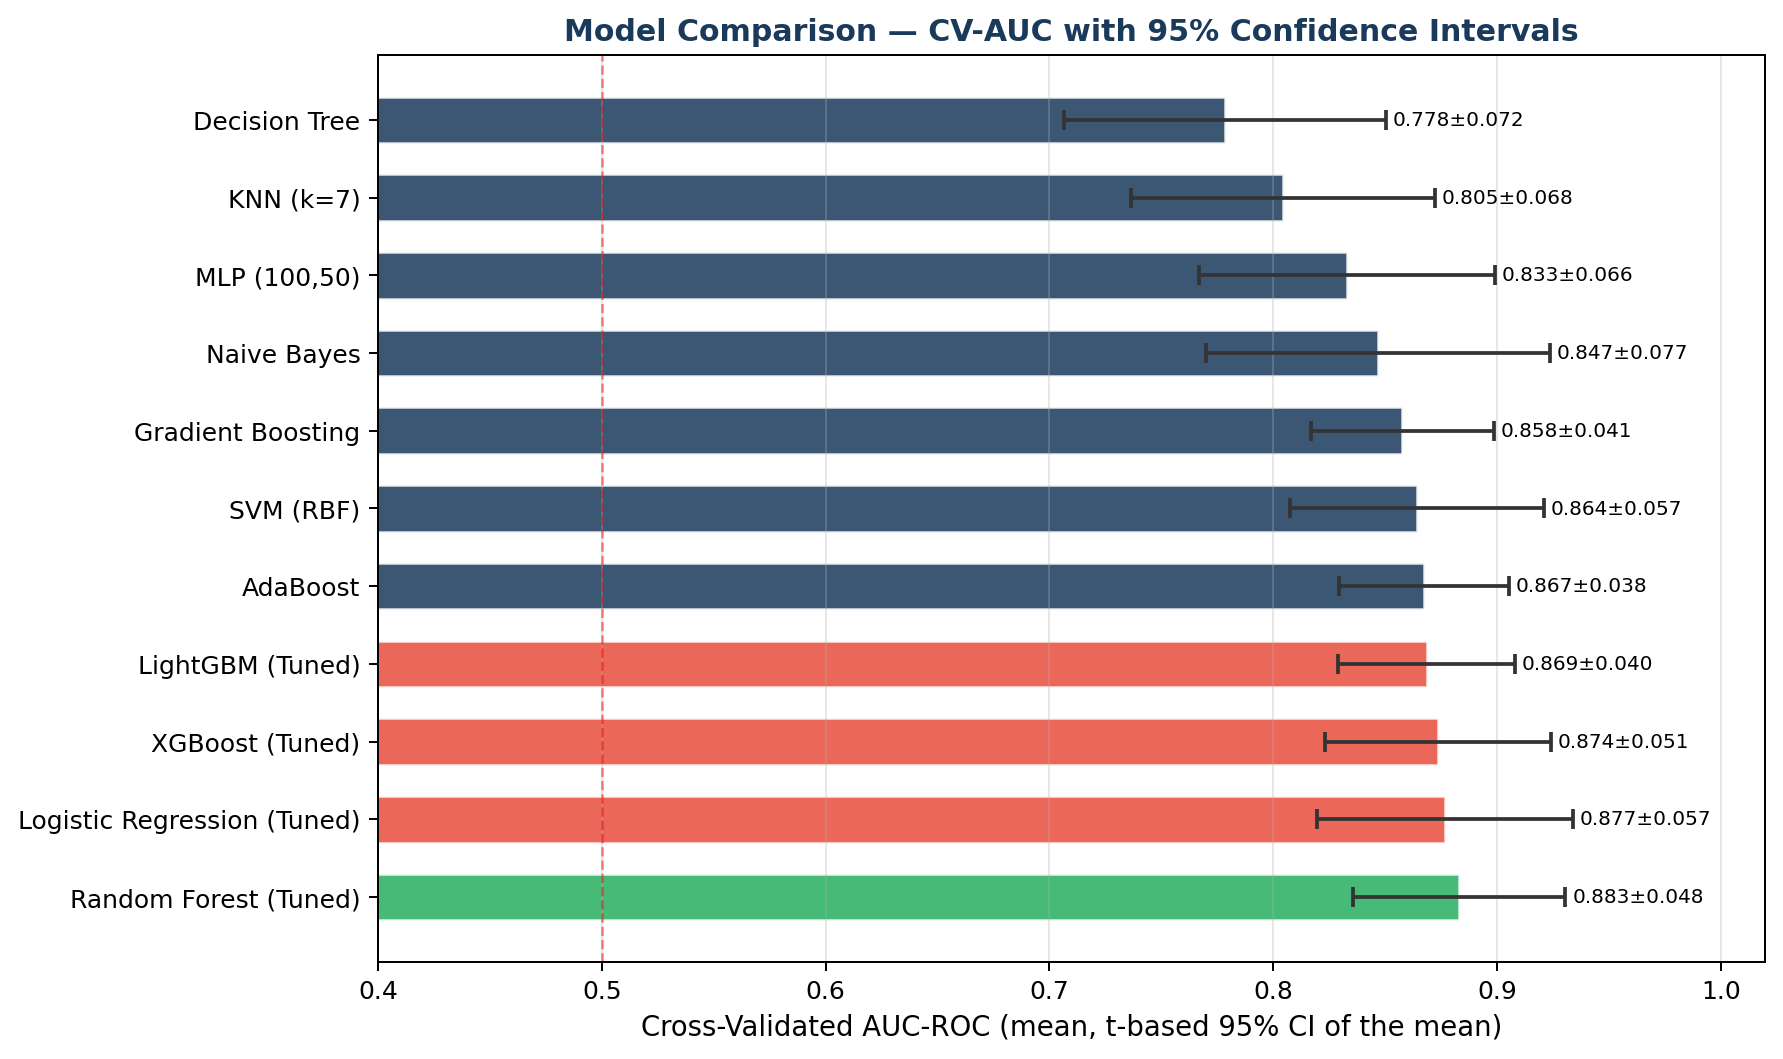
\includegraphics[width=0.78\textwidth]{fig03.png}
\caption{Cross-validated AUC with 95\% confidence intervals (t-based interval of the mean over five outer folds), ranked by mean CV-AUC. Tuned models are shown in red and the selected model in green; tuned models use nested CV.}
\label{fig:3}
\end{figure*}

\begin{figure*}[tbp]
\centering
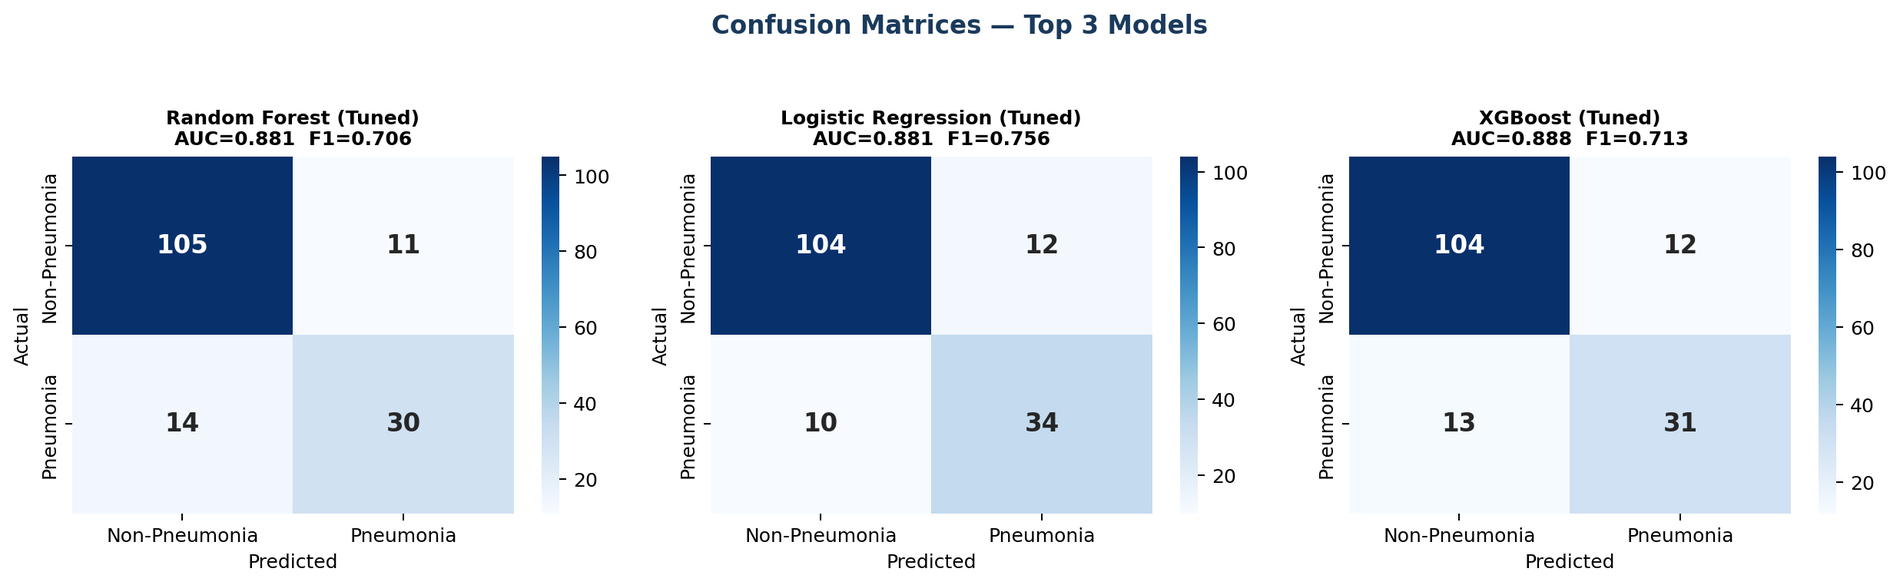
\includegraphics[width=\textwidth]{fig04.png}
\caption{Confusion matrices at threshold 0.5 for the three models with the highest CV-AUC on the held-out test set (n = 160).}
\label{fig:4}
\end{figure*}

\begin{table*}[tbp]
\caption{Performance of all 11 models. Accuracy, precision, recall and F1 are on the held-out test set at threshold 0.5 (n = 160, 44 positive). AUC is test-set AUC with 95\% bootstrap CI (2,000 resamples). CV-AUC is the mean (95\% CI of the mean) over five outer folds on the training set; “Nested” = the complete tuning search was repeated within each fold, “Plain” = fixed-setting model. Models are ordered by CV-AUC.}
\label{tab:4}
\centering
{\scriptsize
\setlength{\tabcolsep}{3.2pt}
\begin{tabular}{>{\raggedright\arraybackslash}p{0.186\textwidth}>{\raggedright\arraybackslash}p{0.060\textwidth}>{\raggedright\arraybackslash}p{0.066\textwidth}>{\raggedright\arraybackslash}p{0.062\textwidth}>{\raggedright\arraybackslash}p{0.053\textwidth}>{\raggedright\arraybackslash}p{0.150\textwidth}>{\raggedright\arraybackslash}p{0.165\textwidth}>{\raggedright\arraybackslash}p{0.131\textwidth}}
\toprule
\textbf{Model} & \textbf{Acc.} & \textbf{Prec.} & \textbf{Recall} & \textbf{F1} & \textbf{Test AUC (95\% CI)} & \textbf{CV-AUC (95\% CI)} & \textbf{CV type} \\
\midrule
Random Forest (Tuned) & 0.844 & 0.732 & 0.682 & 0.706 & 0.881 (0.809--0.938) & 0.883 (0.836--0.931) & Nested \\
Logistic Regression (Tuned) & 0.863 & 0.739 & 0.773 & 0.756 & 0.881 (0.812--0.938) & 0.877 (0.820--0.934) & Nested \\
XGBoost (Tuned) & 0.844 & 0.721 & 0.705 & 0.713 & 0.888 (0.822--0.942) & 0.874 (0.823--0.924) & Nested \\
LightGBM (Tuned) & 0.850 & 0.750 & 0.682 & 0.714 & 0.877 (0.806--0.937) & 0.869 (0.829--0.908) & Nested \\
AdaBoost & 0.844 & 0.721 & 0.705 & 0.713 & 0.873 (0.804--0.934) & 0.867 (0.830--0.905) & Plain \\
SVM (RBF) & 0.838 & 0.750 & 0.614 & 0.675 & 0.863 (0.792--0.926) & 0.864 (0.808--0.921) & Plain \\
Gradient Boosting & 0.825 & 0.690 & 0.659 & 0.674 & 0.849 (0.775--0.915) & 0.858 (0.817--0.899) & Plain \\
Naive Bayes & 0.769 & 0.566 & 0.682 & 0.619 & 0.807 (0.719--0.886) & 0.847 (0.770--0.924) & Plain \\
MLP (100,50) & 0.844 & 0.744 & 0.659 & 0.699 & 0.831 (0.746--0.909) & 0.833 (0.767--0.899) & Plain \\
KNN (k=7) & 0.781 & 0.576 & 0.773 & 0.660 & 0.828 (0.754--0.894) & 0.805 (0.737--0.872) & Plain \\
Decision Tree & 0.800 & 0.607 & 0.773 & 0.680 & 0.796 (0.702--0.885) & 0.778 (0.707--0.850) & Plain \\
\bottomrule
\end{tabular}}
\end{table*}

Random forest, logistic regression, the four boosted-tree models and the SVM clustered at the top (CV-AUC 0.858--0.883), whereas k-nearest neighbours, the single decision tree, the neural network and naive Bayes were clearly lower (0.778--0.847). Two points about the evidence are worth stating. First, the optimism introduced by tuning was small: the inner tuning-CV AUC exceeded the nested CV-AUC by only 0.003 (Random Forest, 0.887 versus 0.883), 0.006 (XGBoost) and 0.009 (LightGBM), and was slightly lower for logistic regression ($-$0.003), suggesting that the search was not materially over-fitted. Second, the seven fixed-setting models were not tuned, so their lower position is partly a statement about default settings and not about the algorithms themselves; the large gap for the decision tree, k-nearest neighbours and naive Bayes is nevertheless consistent with the known advantage of ensembles on small, noisy tabular data. Recall at the default threshold ranged from 0.614 to 0.773. Logistic regression, k-nearest neighbours and the decision tree had the highest recall (0.773), and Random Forest 0.682, so a threshold below 0.5 would be needed if sensitivity is prioritized in screening; this was not tuned here.

The consistent competitiveness of logistic regression with the ensemble methods suggests that the main feature--outcome relationships are approximately linear in the standardized feature space, which supports the use of a transparent points score (see below).

\subsection{Statistical model comparison: DeLong and McNemar tests}

Table~\ref{tab:5} and Fig.~\ref{fig:5} present pairwise comparisons of the four leading models. All DeLong and McNemar tests were non-significant (smallest p = 0.299 for AUC and 0.549 for predictions). Random Forest and logistic regression happened to have identical test AUC (0.8809), so the DeLong statistic is exactly zero for that pair. The AUC differences among the top four models (0.877--0.888 on the test set) are therefore within sampling variability on this test set. Absence of significance is not proof of equivalence in a test set of 160 children, but it indicates that the choice among these candidates should rest on secondary criteria such as calibration, interpretability, and deployment context and not on AUC alone.

\begin{table*}[tbp]
\caption{Pairwise DeLong (AUC) and McNemar (predictions at threshold 0.5) tests on the held-out test set. $\Delta$AUC = AUC of the first minus the second model. b / c are the discordant pairs (first correct and second wrong / first wrong and second correct); McNemar p-values are exact. No comparison was significant.}
\label{tab:5}
\centering
{\scriptsize
\setlength{\tabcolsep}{3.2pt}
\begin{tabular}{>{\raggedright\arraybackslash}p{0.302\textwidth}>{\raggedright\arraybackslash}p{0.102\textwidth}>{\raggedright\arraybackslash}p{0.102\textwidth}>{\raggedright\arraybackslash}p{0.102\textwidth}>{\raggedright\arraybackslash}p{0.144\textwidth}>{\raggedright\arraybackslash}p{0.150\textwidth}}
\toprule
\textbf{Comparison} & \textbf{$\Delta$AUC} & \textbf{DeLong Z} & \textbf{DeLong p} & \textbf{McNemar b / c} & \textbf{McNemar p} \\
\midrule
Random Forest vs. Logistic Regression & 0.000 & 0.000 & 1.000 & 4 / 7 & 0.549 \\
Random Forest vs. XGBoost & $-$0.007 & $-$0.813 & 0.416 & 3 / 3 & 1.000 \\
Random Forest vs. LightGBM & 0.004 & 0.312 & 0.755 & 3 / 4 & 1.000 \\
Logistic Regression vs. XGBoost & $-$0.007 & $-$0.587 & 0.557 & 7 / 4 & 0.549 \\
Logistic Regression vs. LightGBM & 0.004 & 0.262 & 0.793 & 8 / 6 & 0.791 \\
XGBoost vs. LightGBM & 0.011 & 1.040 & 0.299 & 2 / 3 & 1.000 \\
\bottomrule
\end{tabular}}
\end{table*}

\begin{figure*}[tbp]
\centering
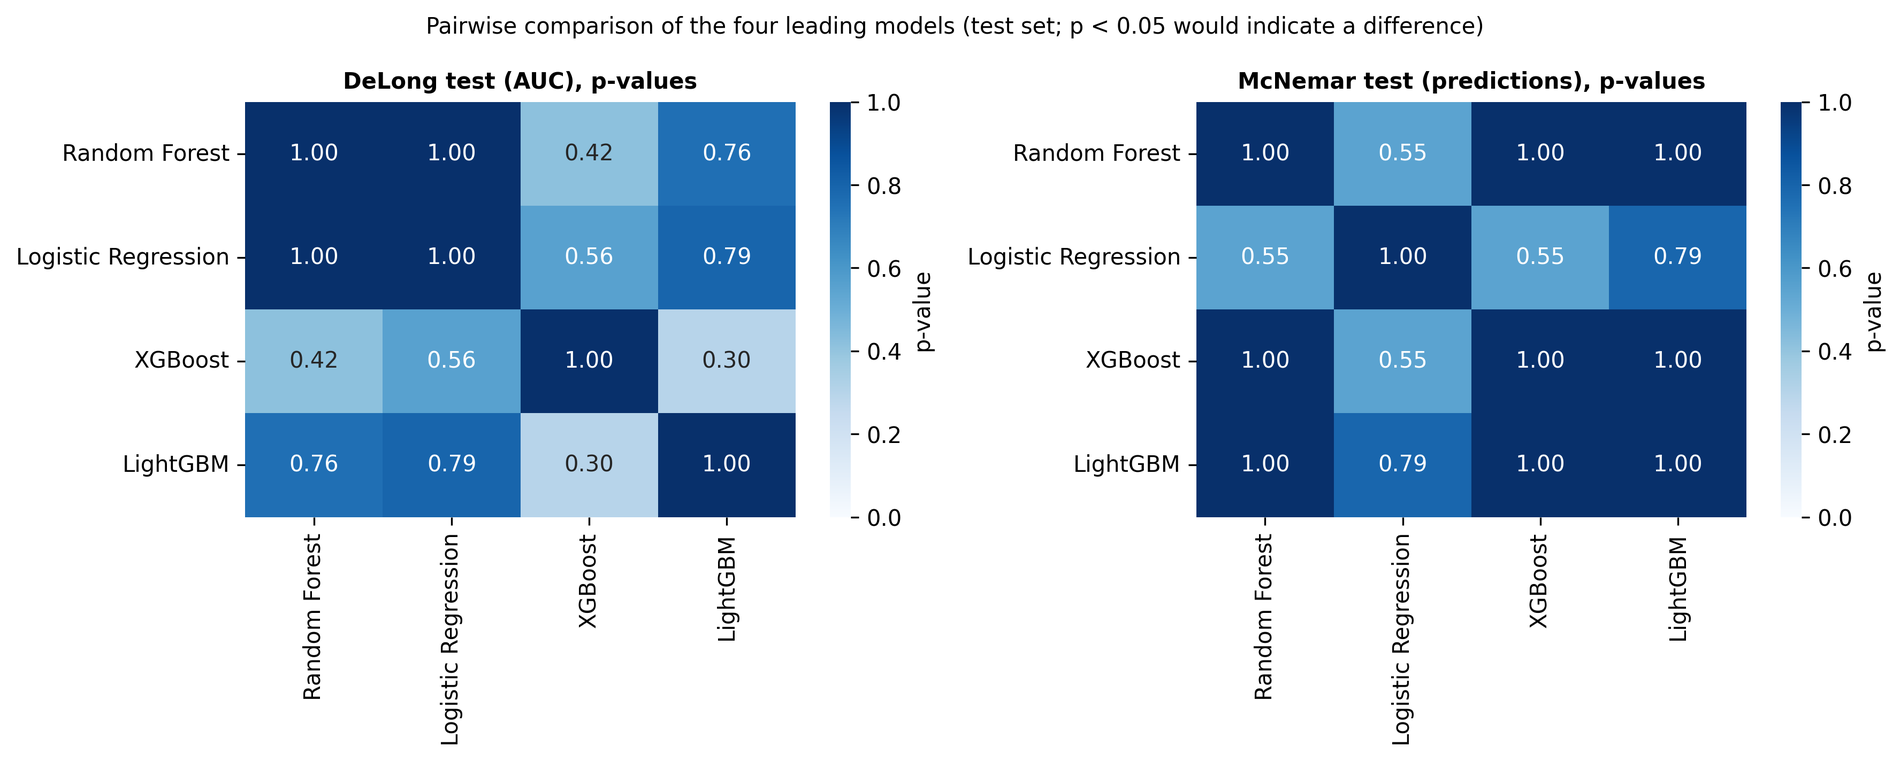
\includegraphics[width=0.88\textwidth]{fig05.png}
\caption{DeLong (left) and McNemar (right) p-value heat maps for the four leading models on the test set. All values exceed 0.05.}
\label{fig:5}
\end{figure*}

\subsection{Probability calibration}
\label{sec:calr}

Table~\ref{tab:6} and Fig.~\ref{fig:6} summarize calibration. The mean predicted probability of the leading models (0.29--0.34) exceeded the observed test prevalence of 0.275, the expected consequence of training on SMOTE-balanced data \cite{r30}; mean predictions were 0.318 for Random Forest, 0.336 for logistic regression, 0.312 for XGBoost and 0.293 for LightGBM. No model was uniformly best calibrated. XGBoost had the lowest Brier score (0.110), LightGBM the lowest ECE (0.048), Random Forest sat in the middle (Brier 0.119, ECE 0.062), and logistic regression had the highest ECE of the four (0.091). AdaBoost, naive Bayes, the neural network and k-nearest neighbours were markedly worse calibrated (ECE 0.15--0.26 for AdaBoost, naive Bayes and the neural network and 0.17 for k-nearest neighbours). With only 44 events and ten bins, the calibration curves in Fig.~\ref{fig:6} are noisy and individual bins contain few patients, so differences of the size seen among the top four should not be over-interpreted. We therefore do not claim that any single model is best calibrated.

\begin{table}[tbp]
\caption{Test-set calibration of all 11 models using raw predicted probabilities (10 equal-width bins), ordered by Brier score. Observed test prevalence = 0.275.}
\label{tab:6}
\centering
{\footnotesize
\setlength{\tabcolsep}{3.2pt}
\begin{tabular}{>{\raggedright\arraybackslash}p{0.350\columnwidth}>{\raggedright\arraybackslash}p{0.160\columnwidth}>{\raggedright\arraybackslash}p{0.160\columnwidth}>{\raggedright\arraybackslash}p{0.198\columnwidth}}
\toprule
\textbf{Model} & \textbf{Brier score} & \textbf{ECE} & \textbf{Mean predicted probability} \\
\midrule
XGBoost (Tuned) & 0.110 & 0.069 & 0.312 \\
LightGBM (Tuned) & 0.113 & 0.048 & 0.293 \\
Random Forest (Tuned) & 0.119 & 0.062 & 0.318 \\
Logistic Regression (Tuned) & 0.119 & 0.091 & 0.336 \\
SVM (RBF) & 0.120 & 0.058 & 0.274 \\
Gradient Boosting & 0.134 & 0.082 & 0.279 \\
MLP (100,50) & 0.146 & 0.150 & 0.250 \\
Decision Tree & 0.148 & 0.112 & 0.321 \\
KNN (k=7) & 0.168 & 0.170 & 0.380 \\
AdaBoost & 0.192 & 0.264 & 0.449 \\
Naive Bayes & 0.195 & 0.201 & 0.328 \\
\bottomrule
\end{tabular}}
\end{table}

\begin{figure*}[tbp]
\centering
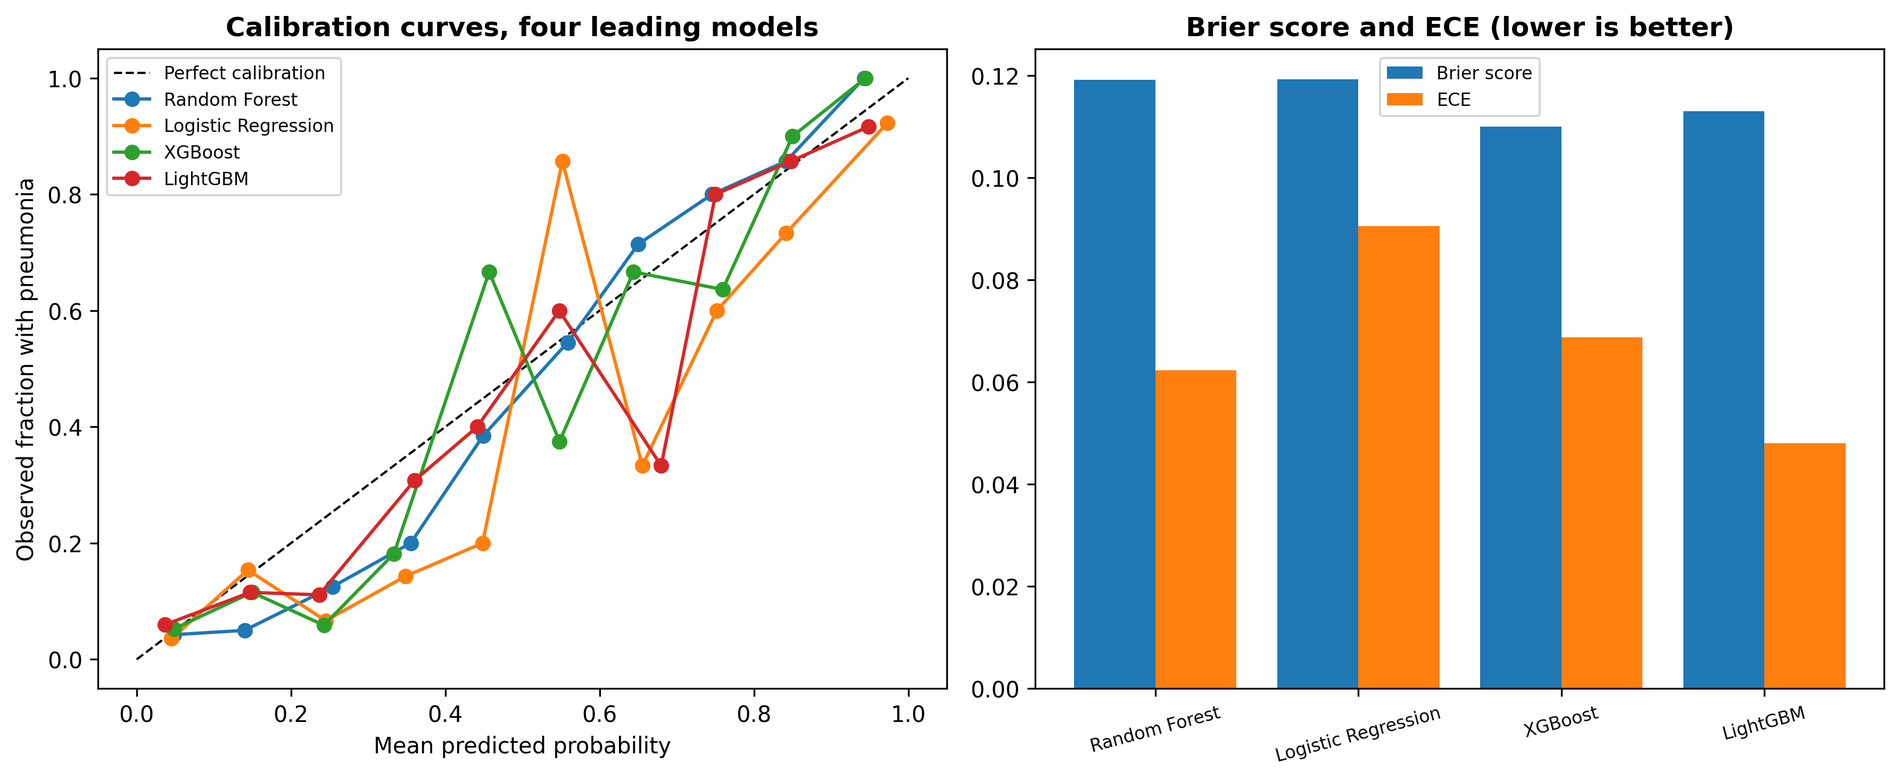
\includegraphics[width=\textwidth]{fig06.png}
\caption{Calibration curves (left) and Brier score / ECE (right) for the four leading models on the test set. Lower values indicate better calibration.}
\label{fig:6}
\end{figure*}

Platt recalibration fitted on training data only produced modest changes (Table~\ref{tab:7}): for Random Forest the Brier score fell from 0.119 to 0.112 with unchanged ECE (0.062) and a negligible change in AUC (0.881 to 0.887); for logistic regression ECE fell from 0.091 to 0.073 while the Brier score and AUC were essentially unchanged (0.121 and 0.874). If predicted probabilities are to be shown to users as absolute risks, recalibration against the target population would be needed; for ranking and triage alone the raw scores suffice.

\begin{table}[tbp]
\caption{Effect of Platt (sigmoid) recalibration on the two models proposed for use (raw $\rightarrow$ recalibrated, test set).}
\label{tab:7}
\centering
{\footnotesize
\setlength{\tabcolsep}{3.2pt}
\begin{tabular}{>{\raggedright\arraybackslash}p{0.287\columnwidth}>{\raggedright\arraybackslash}p{0.192\columnwidth}>{\raggedright\arraybackslash}p{0.192\columnwidth}>{\raggedright\arraybackslash}p{0.198\columnwidth}}
\toprule
\textbf{Model} & \textbf{Brier score} & \textbf{ECE} & \textbf{AUC} \\
\midrule
Random Forest (Tuned) & 0.119 $\rightarrow$ 0.112 & 0.062 $\rightarrow$ 0.062 & 0.881 $\rightarrow$ 0.887 \\
Logistic Regression (Tuned) & 0.119 $\rightarrow$ 0.121 & 0.091 $\rightarrow$ 0.073 & 0.881 $\rightarrow$ 0.874 \\
\bottomrule
\end{tabular}}
\end{table}

\subsection{Decision curve analysis}

Fig.~\ref{fig:7} shows that the four leading models had positive net benefit and exceeded the treat-none strategy at every threshold up to 0.80 and exceeded treat-all at every threshold above about 0.06 on the test set; at a few very low thresholds (0.02--0.06) Random Forest, XGBoost and LightGBM fell marginally below treat-all, whereas logistic regression did not. At a threshold of 0.20, net benefit was 0.175 (Random Forest), 0.175 (logistic regression), 0.177 (XGBoost) and 0.184 (LightGBM), against 0.094 for treat-all; at 0.30 the corresponding values were 0.154, 0.162, 0.170 and 0.166 against $-$0.036 for treat-all, which becomes harmful above a threshold of about 0.27 (the prevalence). At very low thresholds the curves converge with treat-all, as expected when almost every child would be referred. The curves for the four models are close to each other and cross repeatedly, consistent with the non-significant DeLong tests, and with 44 events the curves are noisy. Net benefit was computed from uncalibrated probabilities; because these are inflated, the nominal thresholds should not be read as exact risk levels.

\begin{figure}[tbp]
\centering
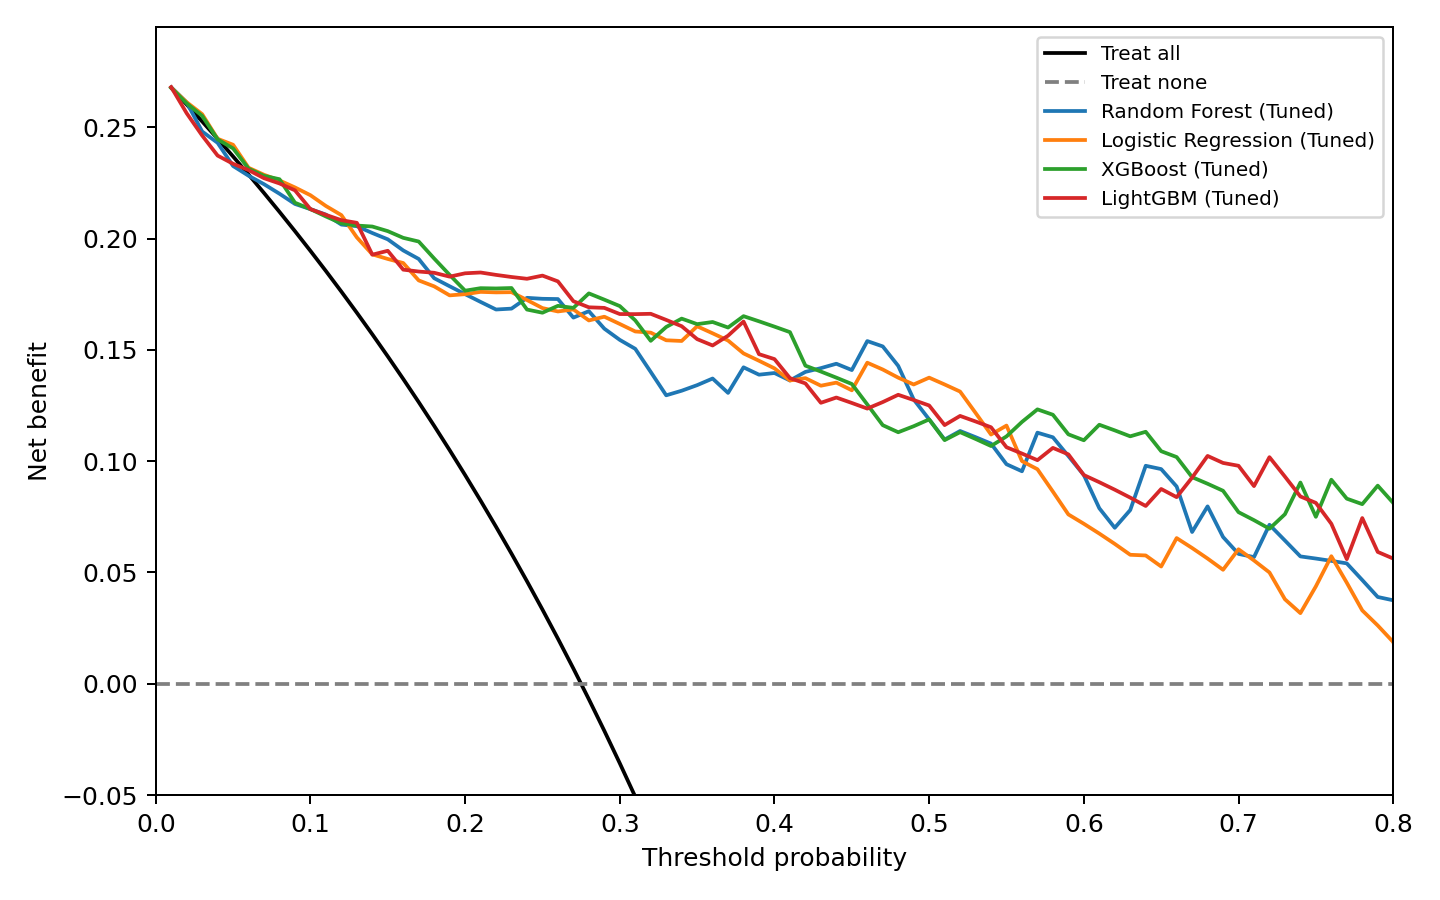
\includegraphics[width=\columnwidth]{fig07.png}
\caption{Decision curve analysis for the four leading models on the test set compared with treat-all and treat-none strategies.}
\label{fig:7}
\end{figure}

\subsection{Feature importance and SHAP analysis}
\label{sec:shap}

Fig.~\ref{fig:8} shows the Random Forest impurity importance and Fig.~\ref{fig:9} the SHAP summary for XGBoost. Wheezing dominated both (Gini importance 0.176; mean |SHAP| 0.905 log-odds), followed by temperature (0.128; 0.464), procalcitonin (0.117; 0.322) and CRP (0.092; 0.279). Grouped by category, Random Forest importance was 75.4\% clinical, 12.8\% demographic, 8.3\% socio-environmental and 3.5\% vaccination. Impurity importance is biased toward continuous variables with many split points and is shown descriptively only.

\begin{figure}[tbp]
\centering
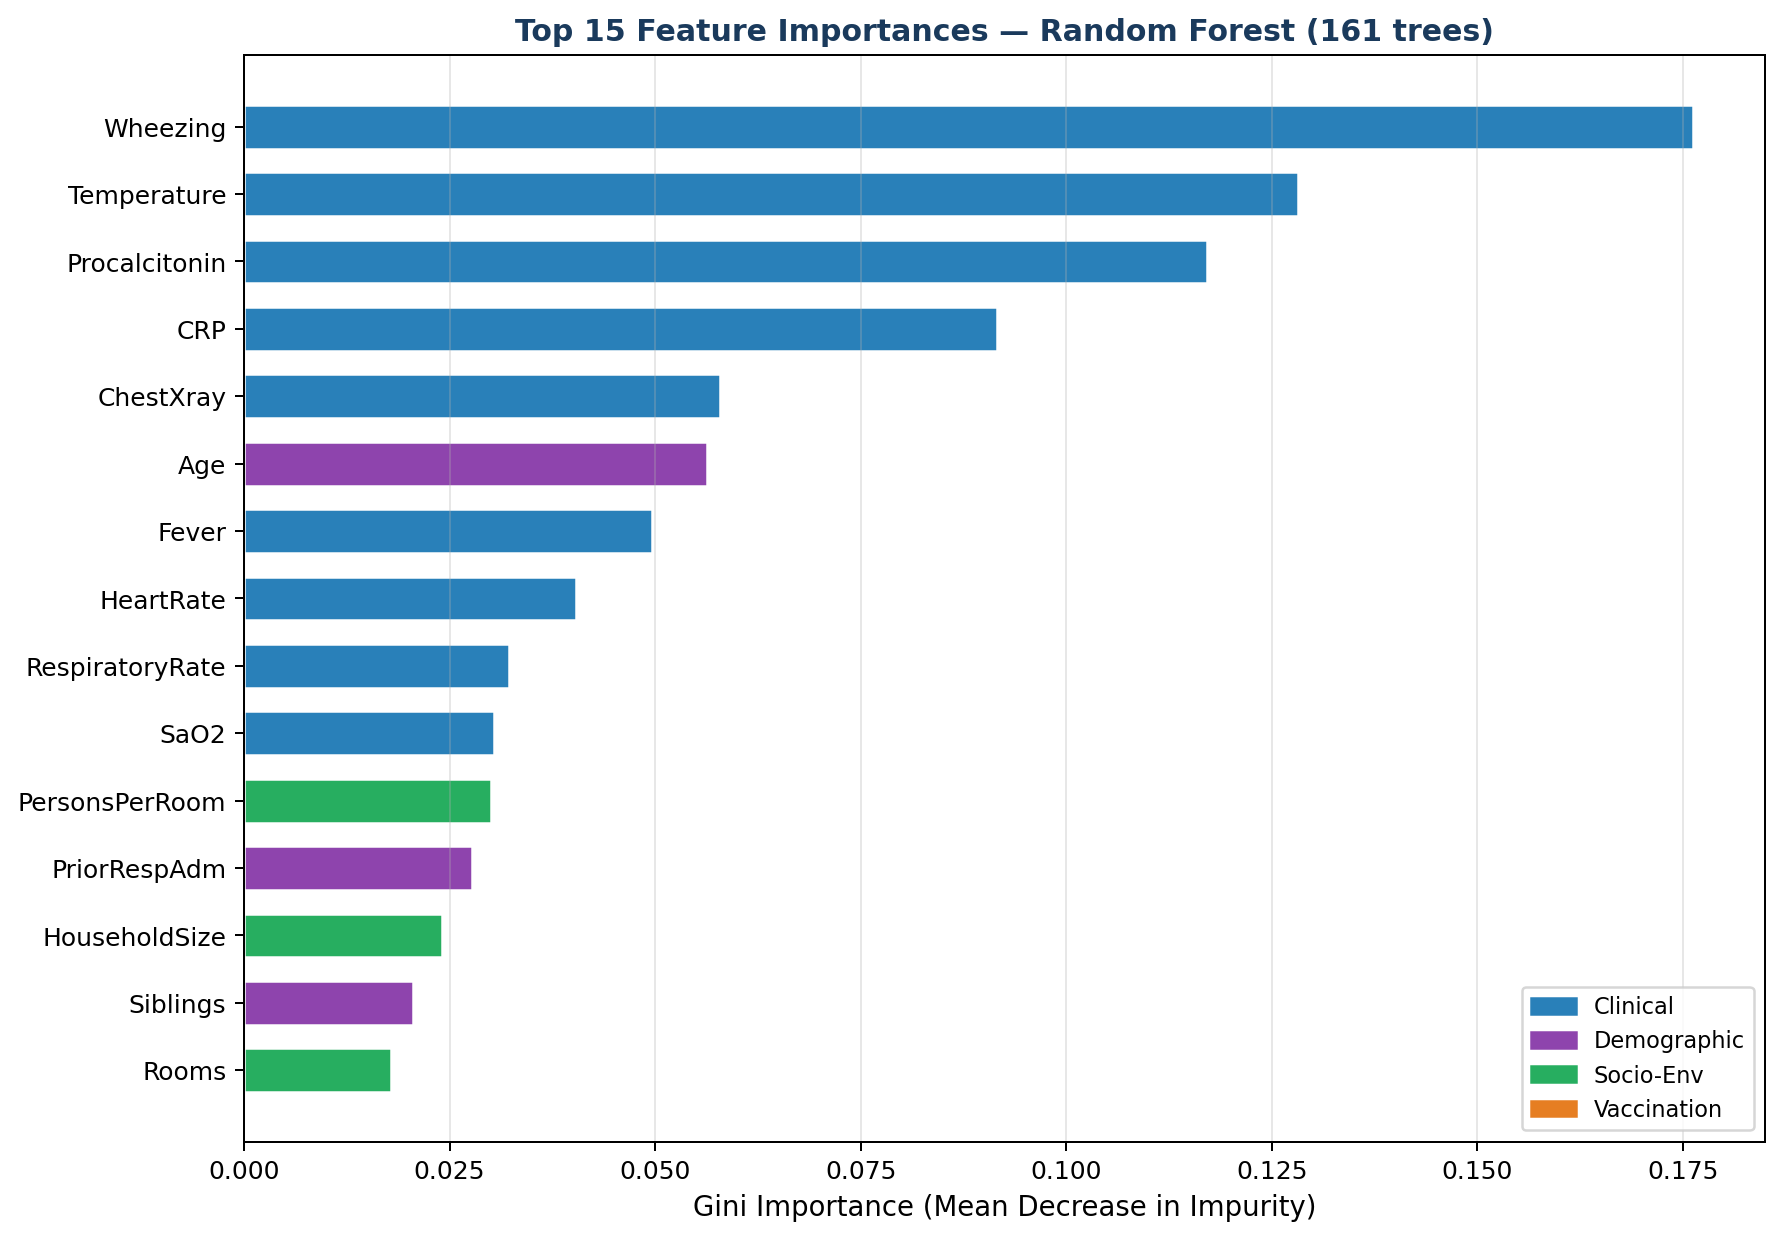
\includegraphics[width=\columnwidth]{fig08.png}
\caption{Top 15 predictors by Gini importance in the tuned Random Forest (161 trees), colour-coded by category.}
\label{fig:8}
\end{figure}

\begin{figure}[tbp]
\centering
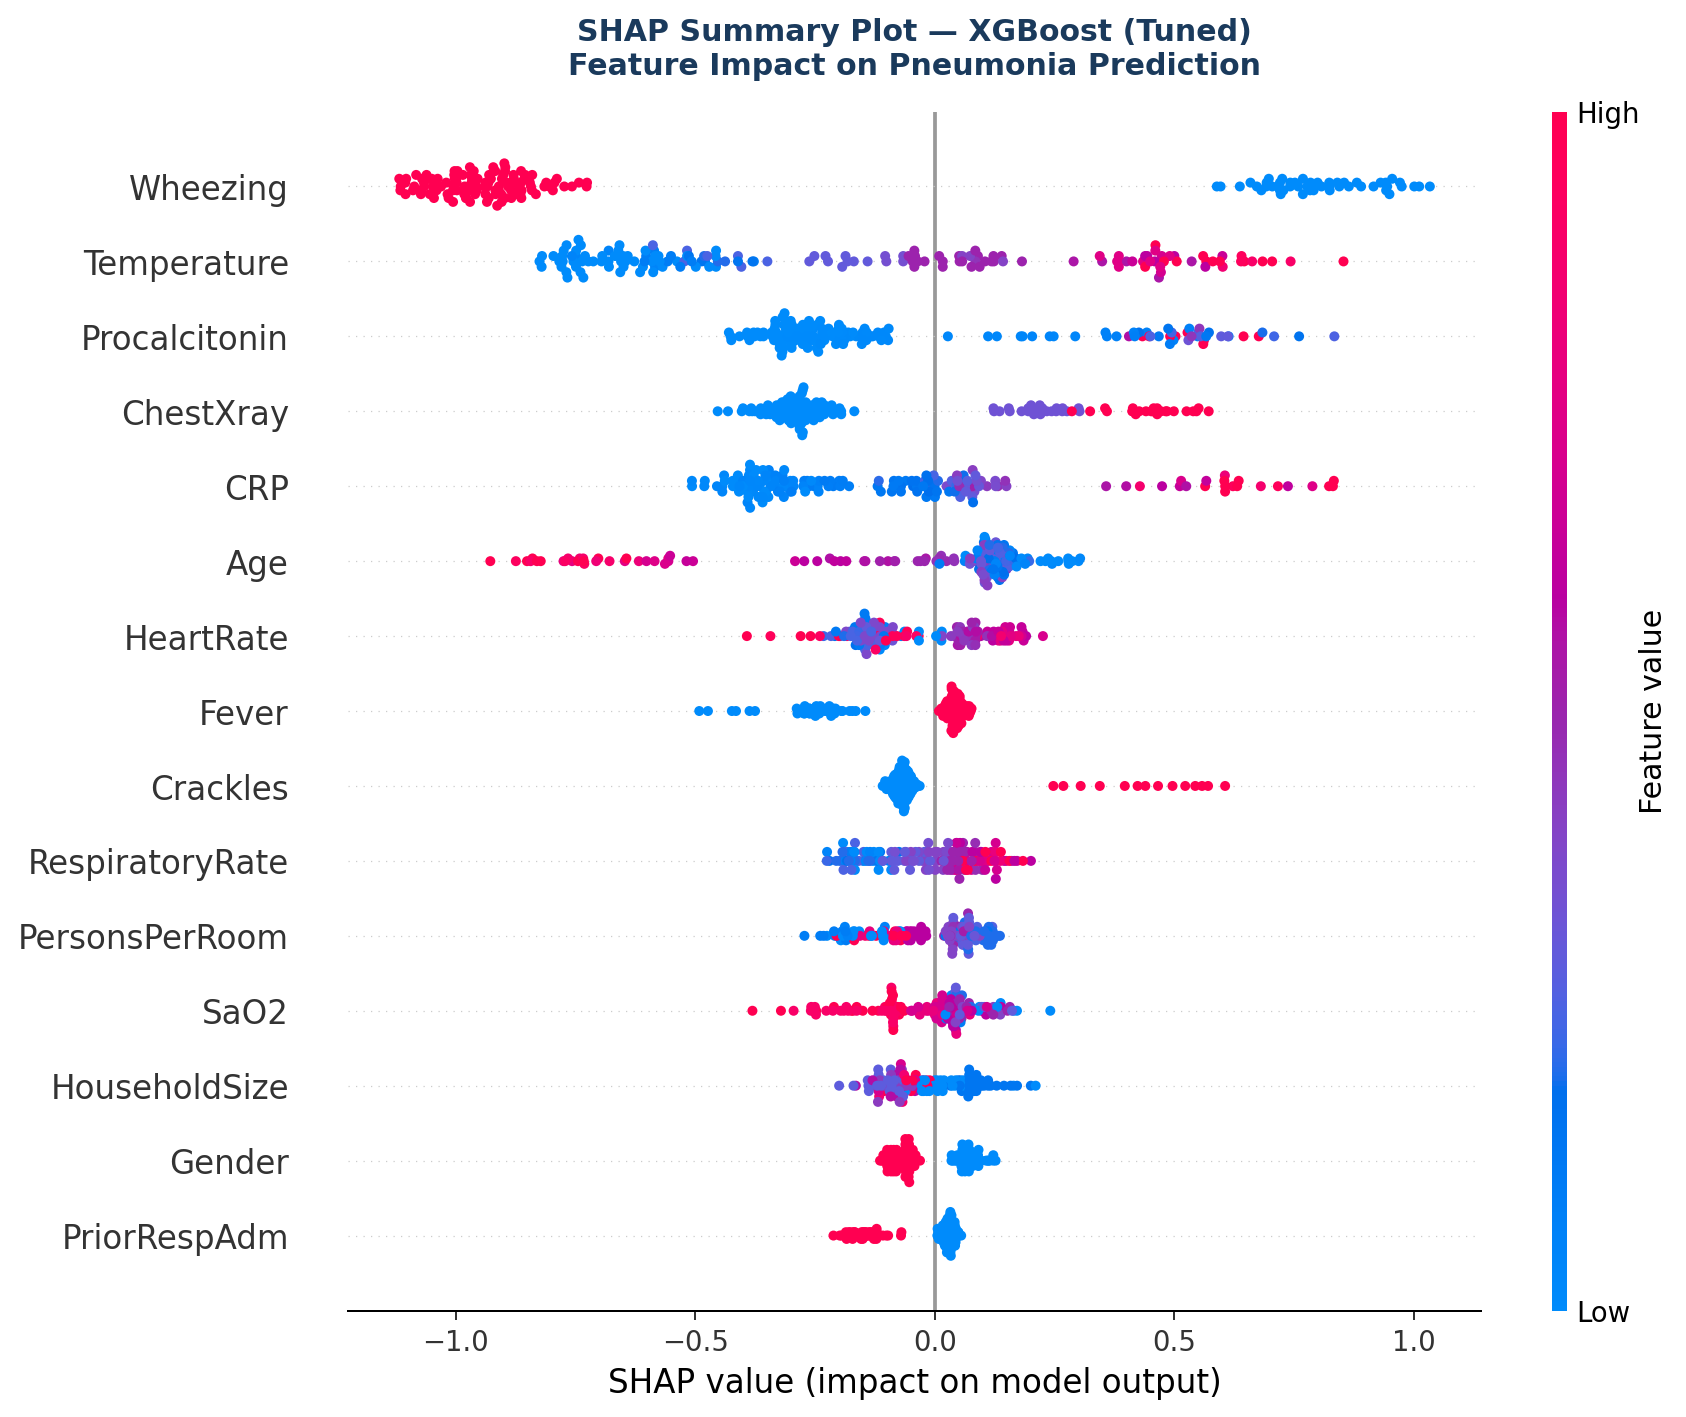
\includegraphics[width=\columnwidth]{fig09.png}
\caption{SHAP summary plot for the tuned XGBoost model on the test set. Colour shows the predictor value (red = high, blue = low); the x-axis is the contribution to the log-odds of a pneumonia label.}
\label{fig:9}
\end{figure}

The direction of the effects, taken from the numerical SHAP table, is as follows. Wheezing was strongly protective: its presence lowered the predicted log-odds on average by 0.95, and its absence raised them by 0.81, reflecting the asthma and bronchiolitis comparison group. Higher temperature, procalcitonin, CRP and a more severe chest X-ray category raised predicted risk (mean SHAP +0.25, +0.22, +0.20 and +0.33 for high values), and older age lowered it ($-$0.26 for above-median age). Crowding behaved differently from the earlier hypothesis: persons-per-room ranked eleventh in mean |SHAP| (0.089) and its mean SHAP value was close to zero for both high and low values ($-$0.013 and $-$0.014), so the model did not use crowding as a consistent directional risk factor. Passive smoking (mean |SHAP| 0.040) and full vaccination (0.027) contributed little once the clinical variables were available. Fig.~\ref{fig:10} shows the dependence plots for the four most influential predictors and Fig.~\ref{fig:11} the explanations for three representative patients. Both figures describe the XGBoost model.

\begin{figure*}[tbp]
\centering
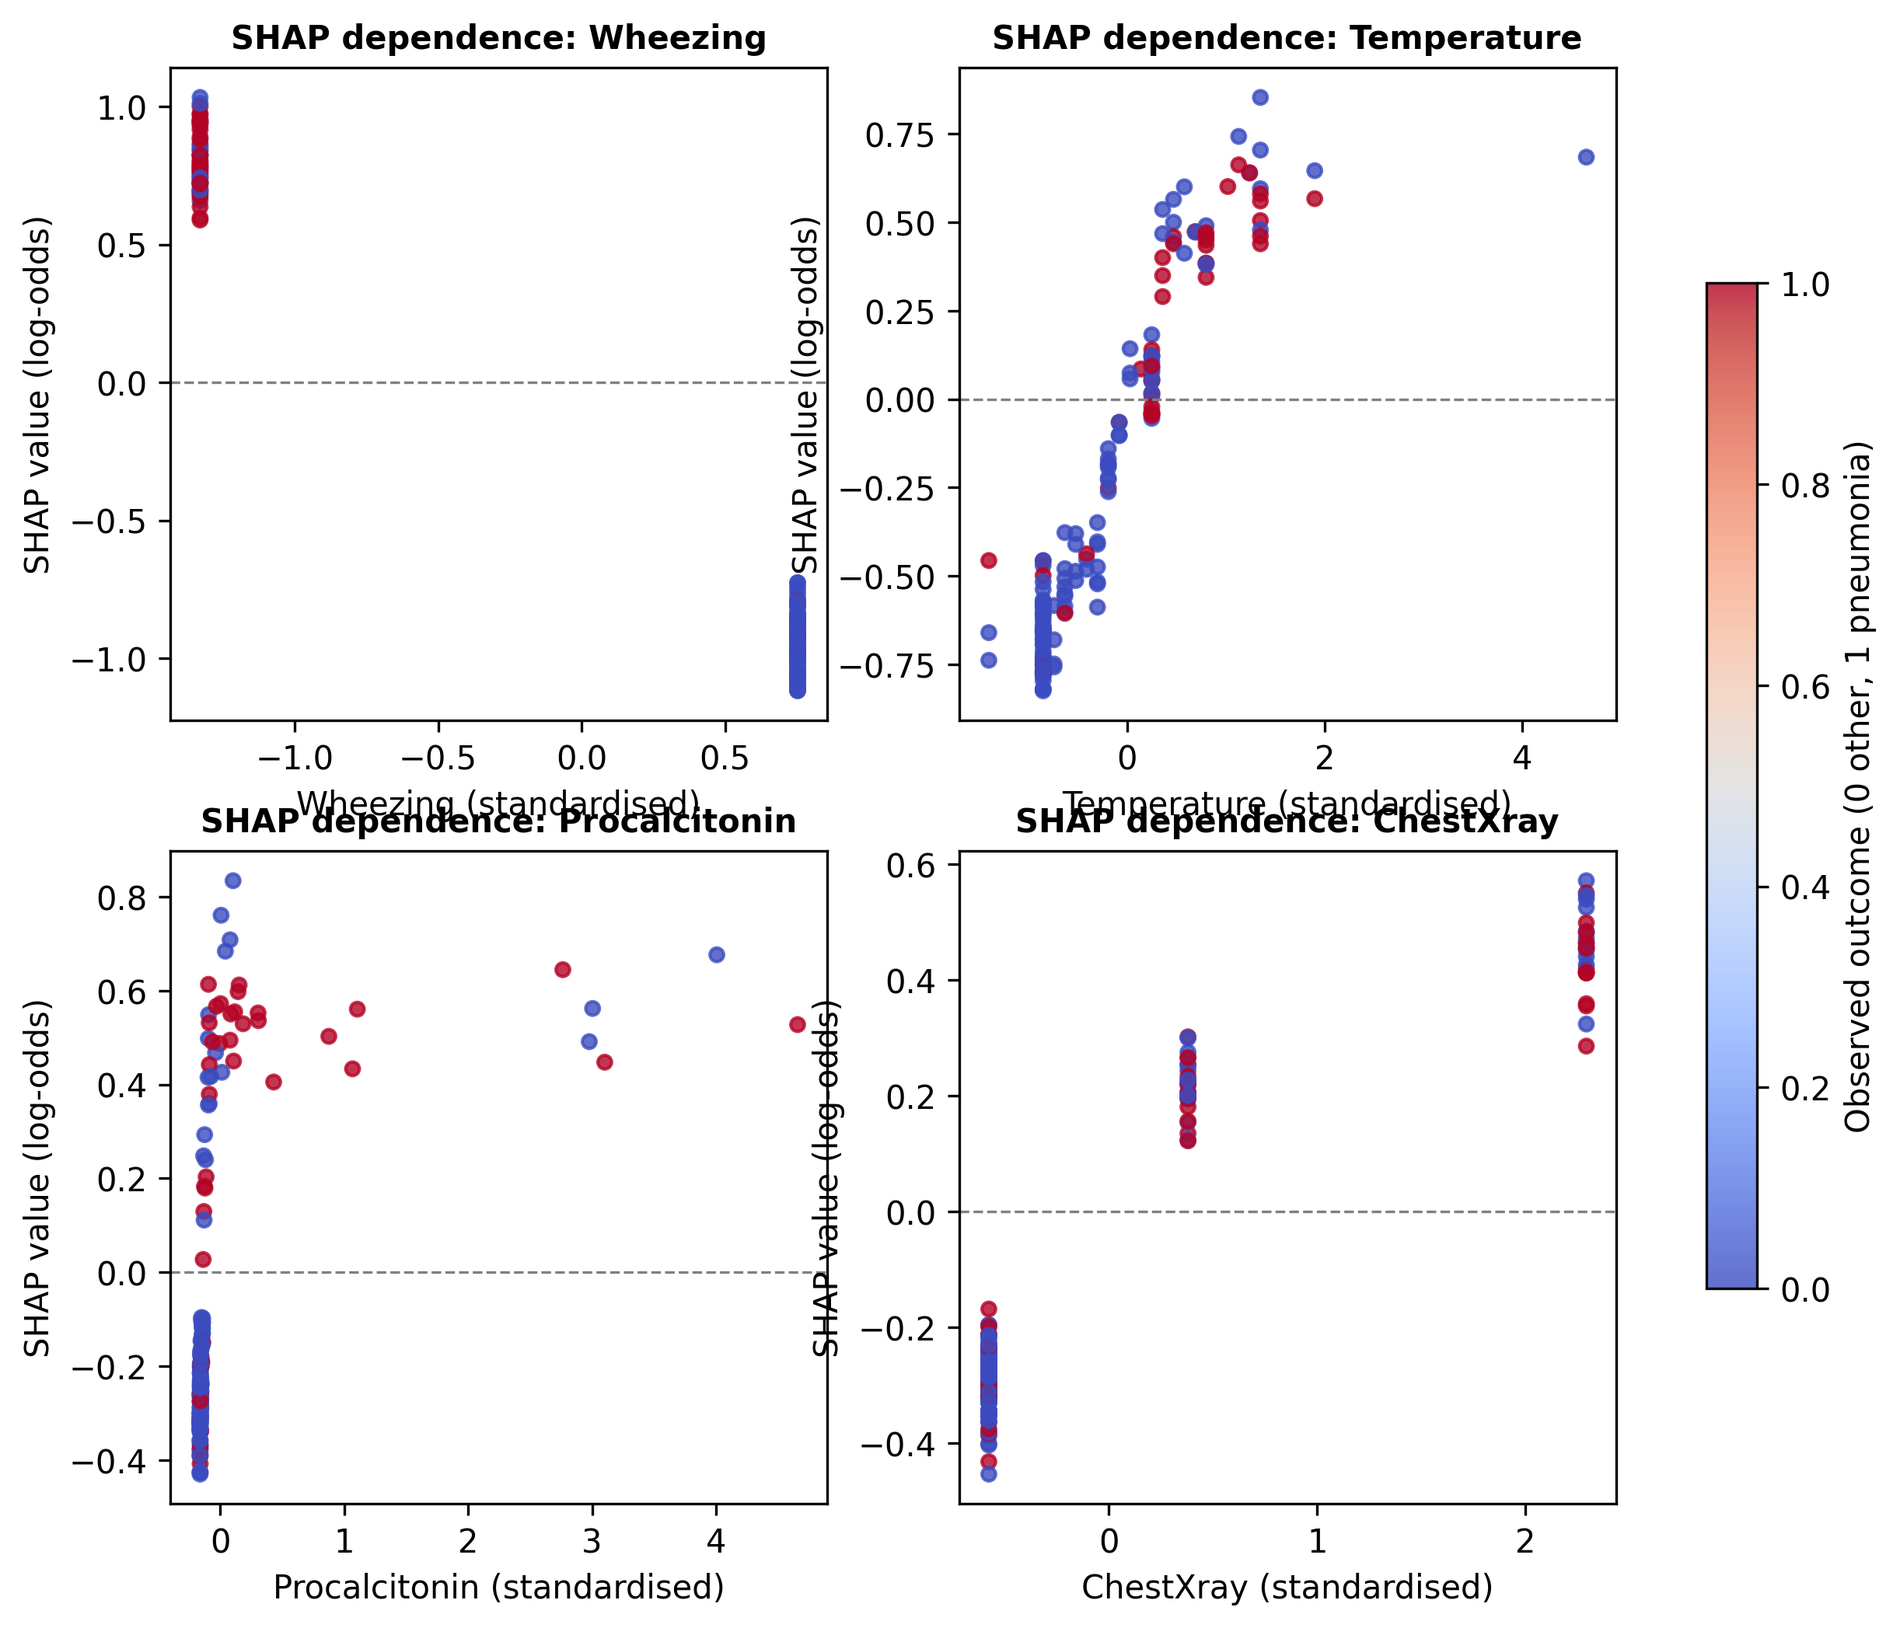
\includegraphics[width=0.66\textwidth]{fig10.png}
\caption{SHAP dependence plots for the four predictors with the largest mean absolute SHAP value (wheezing, temperature, procalcitonin, chest X-ray; XGBoost, test set). Predictor values are standardized; points are coloured by observed outcome.}
\label{fig:10}
\end{figure*}

\begin{figure*}[tbp]
\centering
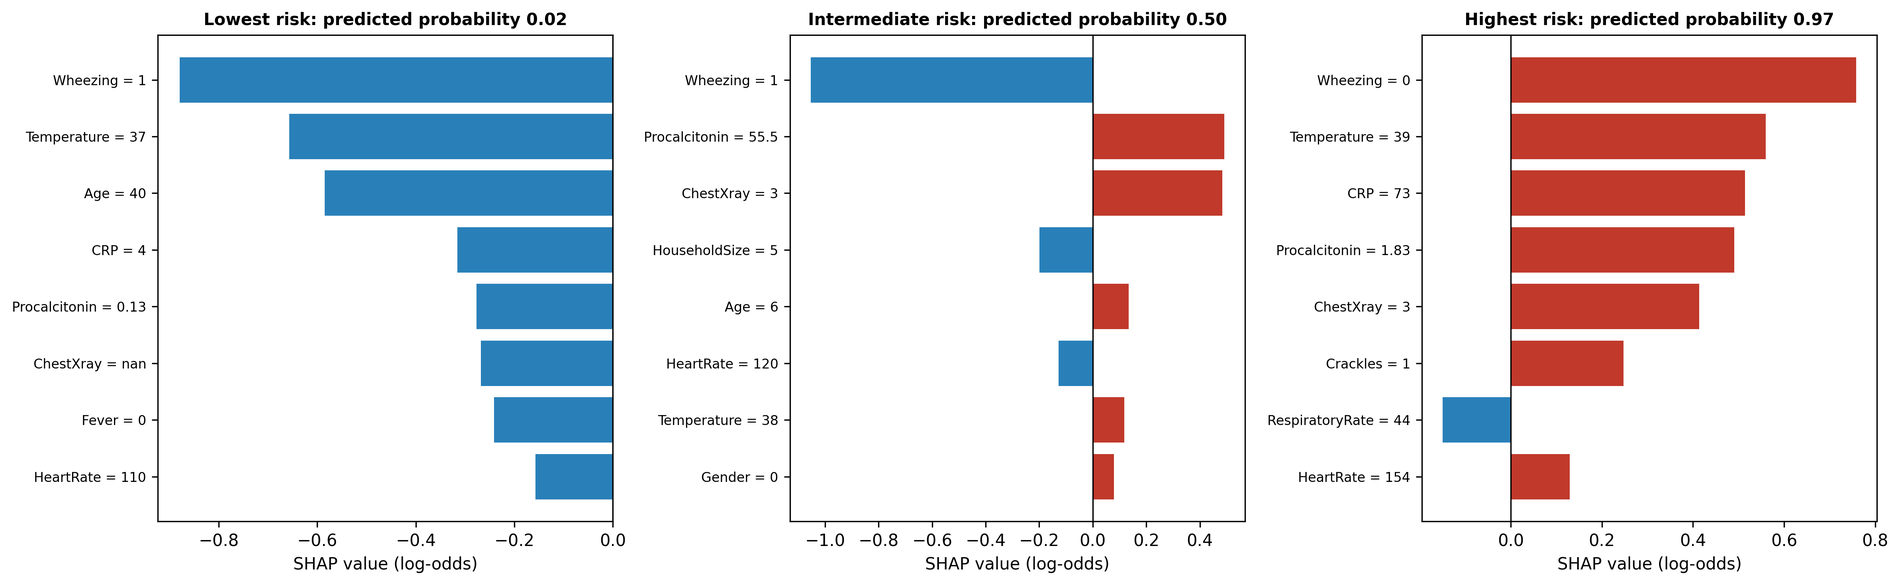
\includegraphics[width=\textwidth]{fig11.png}
\caption{SHAP explanations for the test patients with the lowest (probability 0.02), closest-to-0.5 and highest (0.97) predicted risk (XGBoost). Red bars increase and blue bars decrease the predicted log-odds.}
\label{fig:11}
\end{figure*}

\begin{table}[tbp]
\caption{Directional SHAP summary for the eight most influential predictors (XGBoost, test set). “High” = above the median (or the value 1 for binary predictors).}
\label{tab:8}
\centering
{\footnotesize
\setlength{\tabcolsep}{3.2pt}
\begin{tabular}{>{\raggedright\arraybackslash}p{0.266\columnwidth}>{\raggedright\arraybackslash}p{0.203\columnwidth}>{\raggedright\arraybackslash}p{0.200\columnwidth}>{\raggedright\arraybackslash}p{0.200\columnwidth}}
\toprule
\textbf{Predictor} & \textbf{Mean |SHAP|} & \textbf{Mean SHAP, high values} & \textbf{Mean SHAP, low values} \\
\midrule
Wheezing & 0.905 & $-$0.95 & +0.81 \\
Temperature & 0.464 & +0.25 & $-$0.62 \\
Procalcitonin & 0.322 & +0.22 & $-$0.30 \\
ChestXray & 0.303 & +0.33 & $-$0.29 \\
CRP & 0.279 & +0.20 & $-$0.33 \\
Age & 0.242 & $-$0.26 & +0.15 \\
HeartRate & 0.123 & +0.04 & $-$0.11 \\
Fever & 0.119 & +0.04 & $-$0.26 \\
\bottomrule
\end{tabular}}
\end{table}

\subsection{Feature ablation study}

Table~\ref{tab:9} and Fig.~\ref{fig:12} (left) present the ablation. The clinical-only baseline (A) achieved CV-AUC 0.872 (95\% CI 0.829--0.915), confirming that clinical biomarkers and signs provide most of the predictive information. Adding demographic variables (B) changed the CV-AUC by +0.006 and vaccination variables (D) by +0.005. Adding the five socio-environmental variables alone (C) changed it by $-$0.002 (paired SD 0.011), that is, no improvement. Using all 28 predictors (E) gave the highest value (0.883), +0.011 over the baseline with a small paired SD (0.005), but the confidence intervals of all five configurations overlap almost completely. We therefore report that, in this cohort, socio-environmental variables did not add measurable discriminative information over clinical variables when considered alone, and that the modest gain of the full model is distributed across categories and is small relative to fold-to-fold variability. An earlier version of this work reported a socio-environmental gain of +0.018; that figure is not reproduced by the leakage-free pipeline and nested design reported here and has been withdrawn.

\begin{table*}[tbp]
\caption{Feature-group ablation with the tuned Random Forest on the training set (5 outer folds, hyperparameters fixed). $\Delta$ = mean paired difference in fold AUC versus configuration A (SD of the paired differences).}
\label{tab:9}
\centering
{\scriptsize
\setlength{\tabcolsep}{3.2pt}
\begin{tabular}{>{\raggedright\arraybackslash}p{0.333\textwidth}>{\raggedright\arraybackslash}p{0.091\textwidth}>{\raggedright\arraybackslash}p{0.123\textwidth}>{\raggedright\arraybackslash}p{0.176\textwidth}>{\raggedright\arraybackslash}p{0.192\textwidth}}
\toprule
\textbf{Configuration} & \textbf{Predictors} & \textbf{CV-AUC} & \textbf{95\% CI} & \textbf{$\Delta$ vs A (SD)} \\
\midrule
A Clinical & 12 & 0.872 & 0.829--0.915 & --- \\
B Clinical + Demographic & 18 & 0.878 & 0.840--0.916 & +0.006 (0.006) \\
C Clinical + Socio-Environmental & 17 & 0.870 & 0.838--0.902 & $-$0.002 (0.011) \\
D Clinical + Vaccination & 17 & 0.877 & 0.832--0.921 & +0.005 (0.007) \\
E All features & 28 & 0.883 & 0.835--0.931 & +0.011 (0.005) \\
\bottomrule
\end{tabular}}
\end{table*}

\subsection{Community-level (CHW) model}

Removing the six predictors that need laboratory tests, radiography, auscultation or pulse oximetry reduced discrimination only moderately (Table~\ref{tab:10}, Fig.~\ref{fig:12} right). For Random Forest, CV-AUC fell from 0.883 to 0.854 and test AUC was 0.854 (95\% CI 0.785--0.917); for logistic regression CV-AUC fell from 0.877 to 0.847 with a test AUC of 0.831 (0.757--0.900). This is the analysis most relevant to community deployment, and it indicates that a clinically credible discrimination can be retained with a reduced predictor set, although the list of CHW-collectable variables still includes signs (wheezing, cyanosis, nasal flaring) and measurements (respiratory rate, temperature) that need training and equipment, and it has not been confirmed with CHWs.

\begin{figure*}[tbp]
\centering
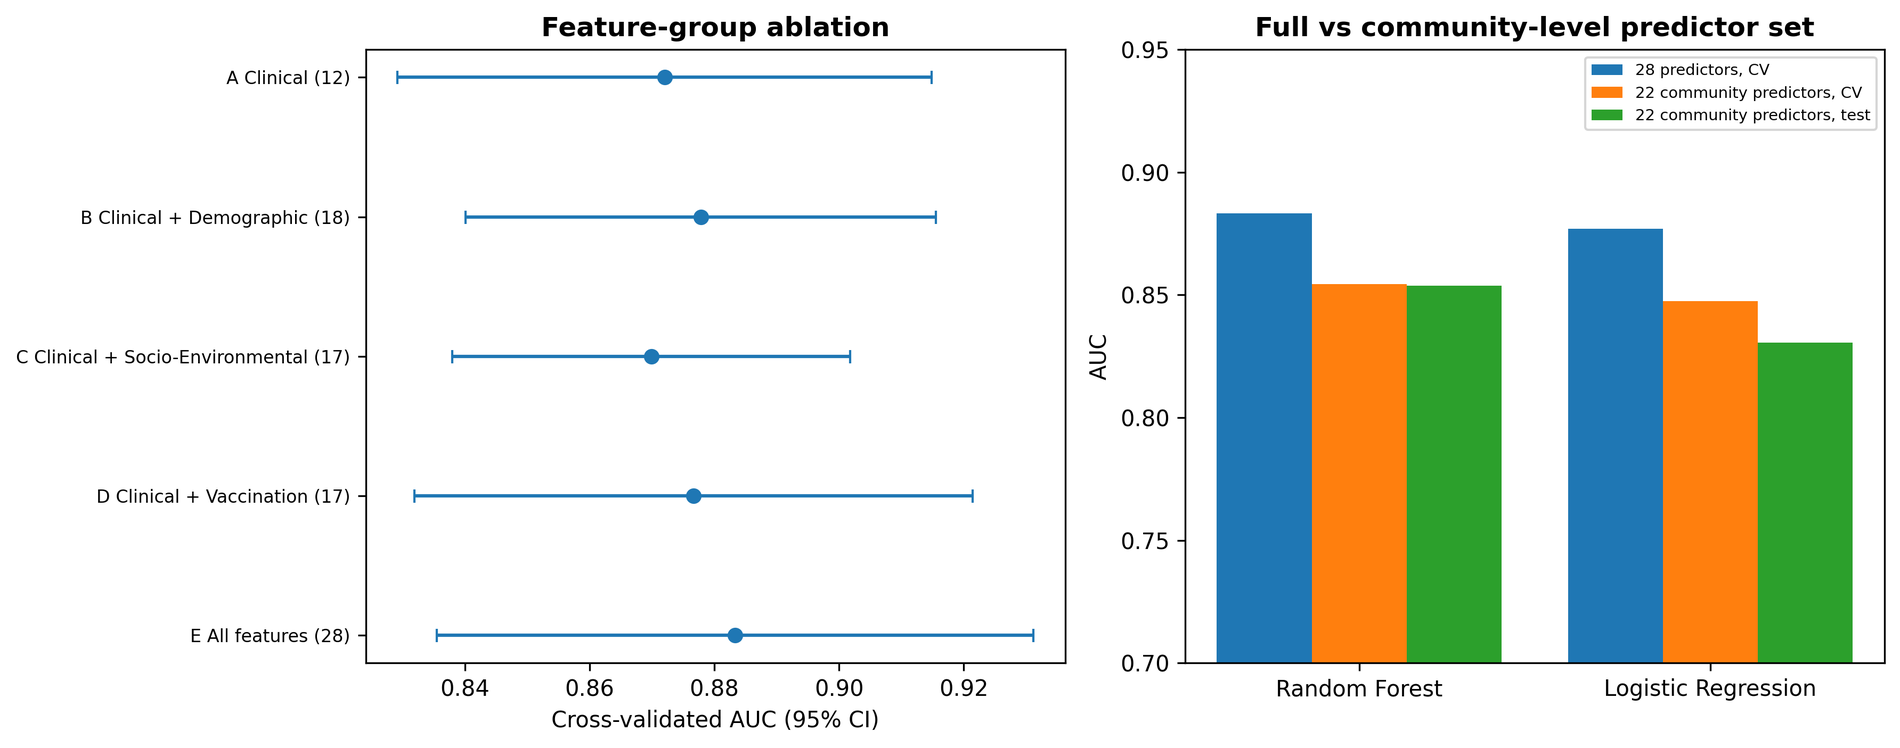
\includegraphics[width=\textwidth]{fig12.png}
\caption{Left: cross-validated AUC (95\% CI) for the five feature-group configurations. Right: full 28-predictor models versus the 22-predictor community-level models (cross-validated and test AUC).}
\label{fig:12}
\end{figure*}

\begin{table*}[tbp]
\caption{Full (28 predictors) versus community-level (22 predictors) models. CV-AUC from five outer folds; test AUC with 95\% bootstrap CI.}
\label{tab:10}
\centering
{\scriptsize
\setlength{\tabcolsep}{3.2pt}
\begin{tabular}{>{\raggedright\arraybackslash}p{0.291\textwidth}>{\raggedright\arraybackslash}p{0.165\textwidth}>{\raggedright\arraybackslash}p{0.165\textwidth}>{\raggedright\arraybackslash}p{0.308\textwidth}}
\toprule
\textbf{Model} & \textbf{Full CV-AUC} & \textbf{CHW CV-AUC} & \textbf{CHW test AUC (95\% CI)} \\
\midrule
Random Forest (Tuned) & 0.883 & 0.854 & 0.854 (0.785--0.917) \\
Logistic Regression (Tuned) & 0.877 & 0.847 & 0.831 (0.757--0.900) \\
\bottomrule
\end{tabular}}
\end{table*}

\subsection{Vaccination, crowding and the Community Exposure Risk Score}

Pneumonia prevalence rose across vaccination categories (Fig.~\ref{fig:13}): 25.2\% (177 of 701) in fully vaccinated, 40.2\% (35 of 87) in partially vaccinated and 57.1\% (4 of 7) in unvaccinated children, consistent with immunological theory and prior epidemiological evidence \cite{r5,r8,r9}. The gradient is monotonic, but the unvaccinated group contains only seven children, so its estimate is highly imprecise, and these are unadjusted proportions that may be confounded, for example by age. Crowding showed little separation between outcome groups (Fig.~\ref{fig:14}; quartile chi-square p = 0.187).

\begin{figure}[tbp]
\centering
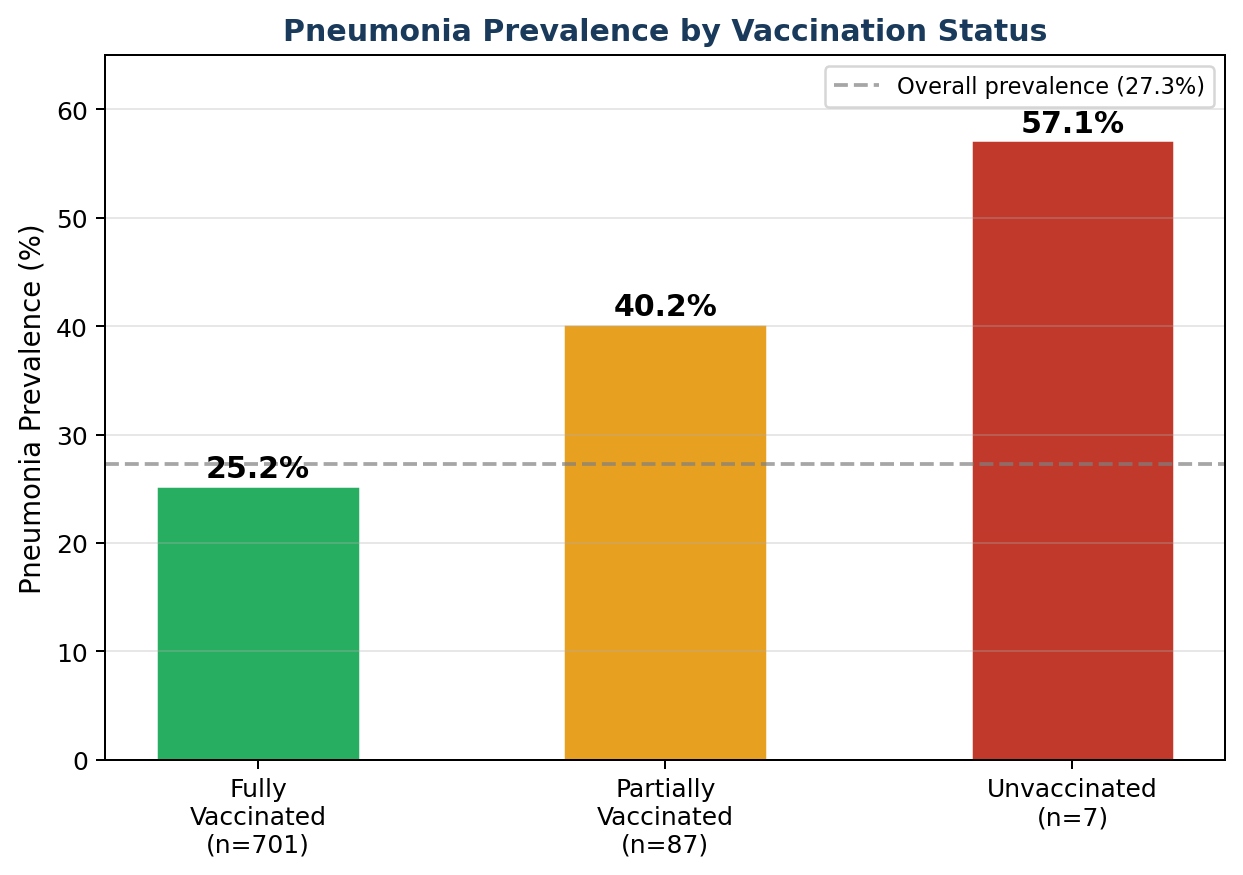
\includegraphics[width=\columnwidth]{fig13.png}
\caption{Pneumonia prevalence by vaccination status. The unvaccinated group contains seven children.}
\label{fig:13}
\end{figure}

\begin{figure*}[tbp]
\centering
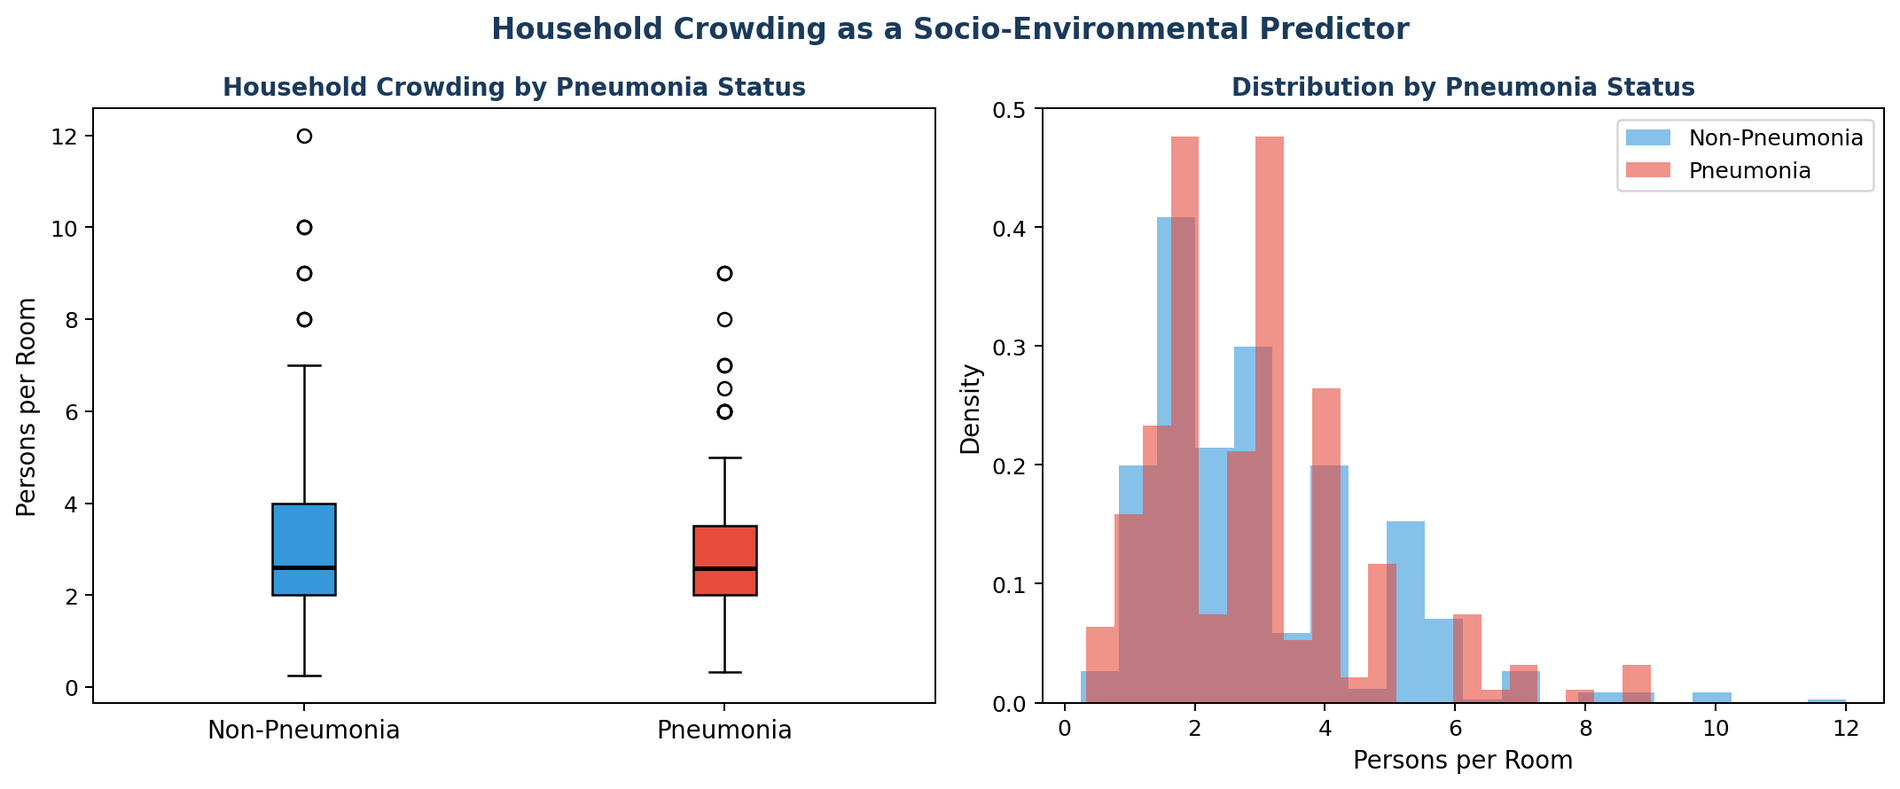
\includegraphics[width=0.9\textwidth]{fig14.png}
\caption{Household crowding (persons per room) by pneumonia status.}
\label{fig:14}
\end{figure*}

Data-driven CERS weights (Table~\ref{tab:11}, Fig.~\ref{fig:15}) gave the dominant weight to vaccination risk (0.698), followed by smoking (0.176) and household size (0.126). Persons-per-room had a negative logistic coefficient ($-$0.64), meaning that, with the other three variables in the model, higher crowding was associated with slightly lower pneumonia odds in this cohort; it was truncated to a weight of zero. The optimized score discriminated poorly on the test set (AUC 0.540) and only marginally better than the expert score (0.532), both close to chance. The CERS therefore did not serve as an effective composite predictor here; its value is in documenting that, in this hospitalized cohort, the community-exposure variables carry little discriminative information once considered together. Because the weights were estimated on the same training data used for model development, and the weights themselves are unstable with so few unvaccinated children, they should not be used as general epidemiological weights.

\begin{table}[tbp]
\caption{CERS weights and discrimination. Raw coefficients from L2-regularized logistic regression on min--max-scaled training data; optimized weights are the truncated, normalized coefficients.}
\label{tab:11}
\centering
{\footnotesize
\setlength{\tabcolsep}{3.2pt}
\begin{tabular}{>{\raggedright\arraybackslash}p{0.308\columnwidth}>{\raggedright\arraybackslash}p{0.182\columnwidth}>{\raggedright\arraybackslash}p{0.182\columnwidth}>{\raggedright\arraybackslash}p{0.198\columnwidth}}
\toprule
\textbf{Variable} & \textbf{Raw LR coefficient} & \textbf{Optimized weight} & \textbf{Expert weight} \\
\midrule
Persons per room & $-$0.641 & 0.000 & 0.350 \\
Smokers at home & 0.297 & 0.176 & 0.300 \\
Vaccination risk (0 / 0.5 / 1) & 1.181 & 0.698 & 0.200 \\
Household size & 0.213 & 0.126 & 0.150 \\
\bottomrule
\end{tabular}}
\vspace{6pt}
{\footnotesize
\begin{tabular}{>{\raggedright\arraybackslash}p{0.308\columnwidth}>{\raggedright\arraybackslash}p{0.295\columnwidth}>{\raggedright\arraybackslash}p{0.295\columnwidth}}
\toprule
\textbf{Score} & \textbf{AUC, training set} & \textbf{AUC, test set} \\
\midrule
Expert CERS & 0.542 & 0.532 \\
Optimized CERS & 0.566 & 0.540 \\
\bottomrule
\end{tabular}}
\end{table}

\begin{figure*}[tbp]
\centering
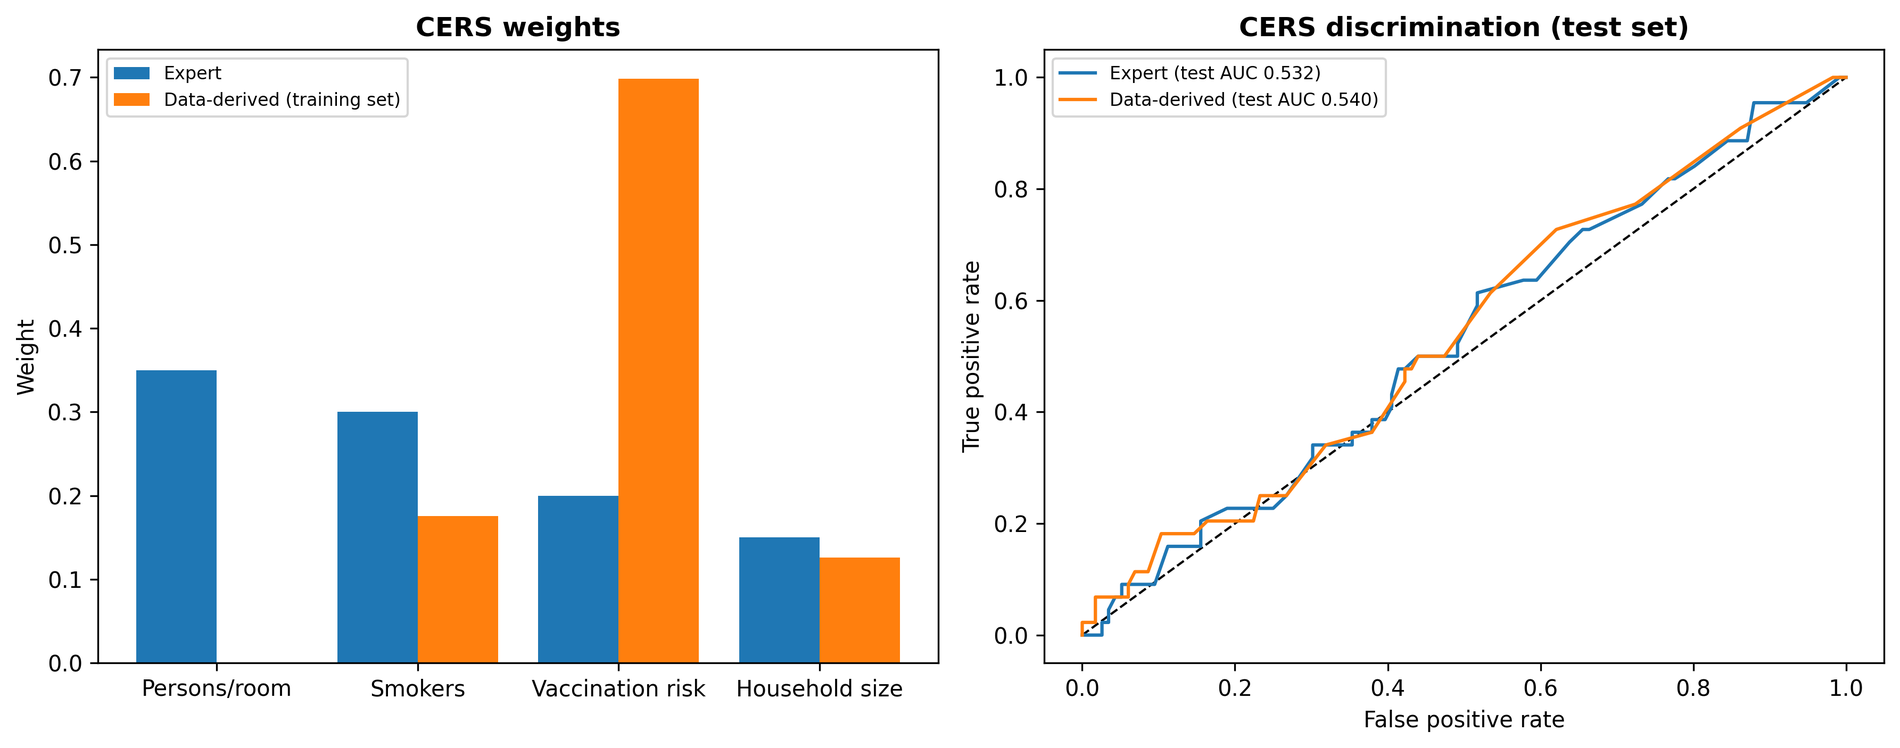
\includegraphics[width=\textwidth]{fig15.png}
\caption{CERS weights (left) and test-set ROC curves for the expert and data-derived scores (right).}
\label{fig:15}
\end{figure*}

\subsection{Community Pneumonia Screening Score (CPSS)}

The CPSS points derived from the training set are shown in Table~\ref{tab:12}. Wheezing carried $-$5 points (odds ratio 0.10), fever +2.5 (OR 3.12), vaccination risk +4 (OR 6.02 for unvaccinated versus fully vaccinated; partial vaccination scores +2) and passive smoking +1 (OR 1.49). Crowding rounded to zero points (OR 0.96) and contributes nothing, so it can be dropped from the score. A child’s score is the sum of applicable points and ranges from $-$5 to +7.5. The score discriminated well on the test set (AUC 0.847, 95\% CI 0.771--0.915; training AUC 0.827). By contrast, the fixed weights proposed in the earlier version of this work (which added points for wheezing) performed worse than chance (test AUC 0.274), because wheezing is protective in this dataset; those weights are replaced here.

\begin{table}[tbp]
\caption{CPSS: logistic regression coefficients on the training set and the resulting points (largest |coefficient| = 5 points, rounded to 0.5).}
\label{tab:12}
\centering
{\footnotesize
\setlength{\tabcolsep}{3.2pt}
\begin{tabular}{>{\raggedright\arraybackslash}p{0.403\columnwidth}>{\raggedright\arraybackslash}p{0.150\columnwidth}>{\raggedright\arraybackslash}p{0.150\columnwidth}>{\raggedright\arraybackslash}p{0.167\columnwidth}}
\toprule
\textbf{Predictor} & \textbf{Log-odds} & \textbf{Odds ratio} & \textbf{Points} \\
\midrule
Wheezing present (0/1) & $-$2.352 & 0.095 & $-$5.0 \\
History of fever (0/1) & 1.139 & 3.124 & +2.5 \\
$\geq$3 persons per room (0/1) & $-$0.041 & 0.960 & 0.0 \\
Vaccination risk (0 full, 0.5 partial, 1 none) & 1.795 & 6.018 & +4.0 \\
Smoker at home (0/1) & 0.400 & 1.492 & +1.0 \\
\bottomrule
\end{tabular}}
\end{table}

Table~\ref{tab:13} and Fig.~\ref{fig:16} show the observed pneumonia rate by score. Rates rose steeply with score: 9.4\% (training) and 7.0\% (test) at scores of $-$1.5 or lower, 21.8\% and 33.3\% for scores from $-$0.5 to 2.0, and 62.1\% and 73.8\% for scores of 2.5 or higher. These bands were described after inspecting the score distribution and are not pre-specified thresholds; the intermediate band in particular is small (55 training and 18 test children) and heterogeneous. They illustrate that the score orders risk sensibly, but cut-offs and the management actions attached to them (for example referral urgency) need to be fixed and validated in an independent sample before the score is used. In this cohort the score is also dominated by the absence of wheezing, which reflects the hospital case-mix and may not hold in community populations where pneumonia must be separated from a different group of illnesses.

\begin{table*}[tbp]
\caption{Observed pneumonia rate by CPSS band (descriptive, post hoc bands).}
\label{tab:13}
\centering
{\scriptsize
\setlength{\tabcolsep}{3.2pt}
\begin{tabular}{>{\raggedright\arraybackslash}p{0.302\textwidth}>{\raggedright\arraybackslash}p{0.102\textwidth}>{\raggedright\arraybackslash}p{0.224\textwidth}>{\raggedright\arraybackslash}p{0.102\textwidth}>{\raggedright\arraybackslash}p{0.186\textwidth}}
\toprule
\textbf{CPSS band} & \textbf{Train n} & \textbf{Train pneumonia} & \textbf{Test n} & \textbf{Test pneumonia} \\
\midrule
Low (score $\leq$ $-$1.5) & 381 & 36 (9.4\%) & 100 & 7 (7.0\%) \\
Intermediate ($-$0.5 to 2.0) & 55 & 12 (21.8\%) & 18 & 6 (33.3\%) \\
High ($\geq$ 2.5) & 203 & 126 (62.1\%) & 42 & 31 (73.8\%) \\
\bottomrule
\end{tabular}}
\end{table*}

\begin{figure*}[tbp]
\centering
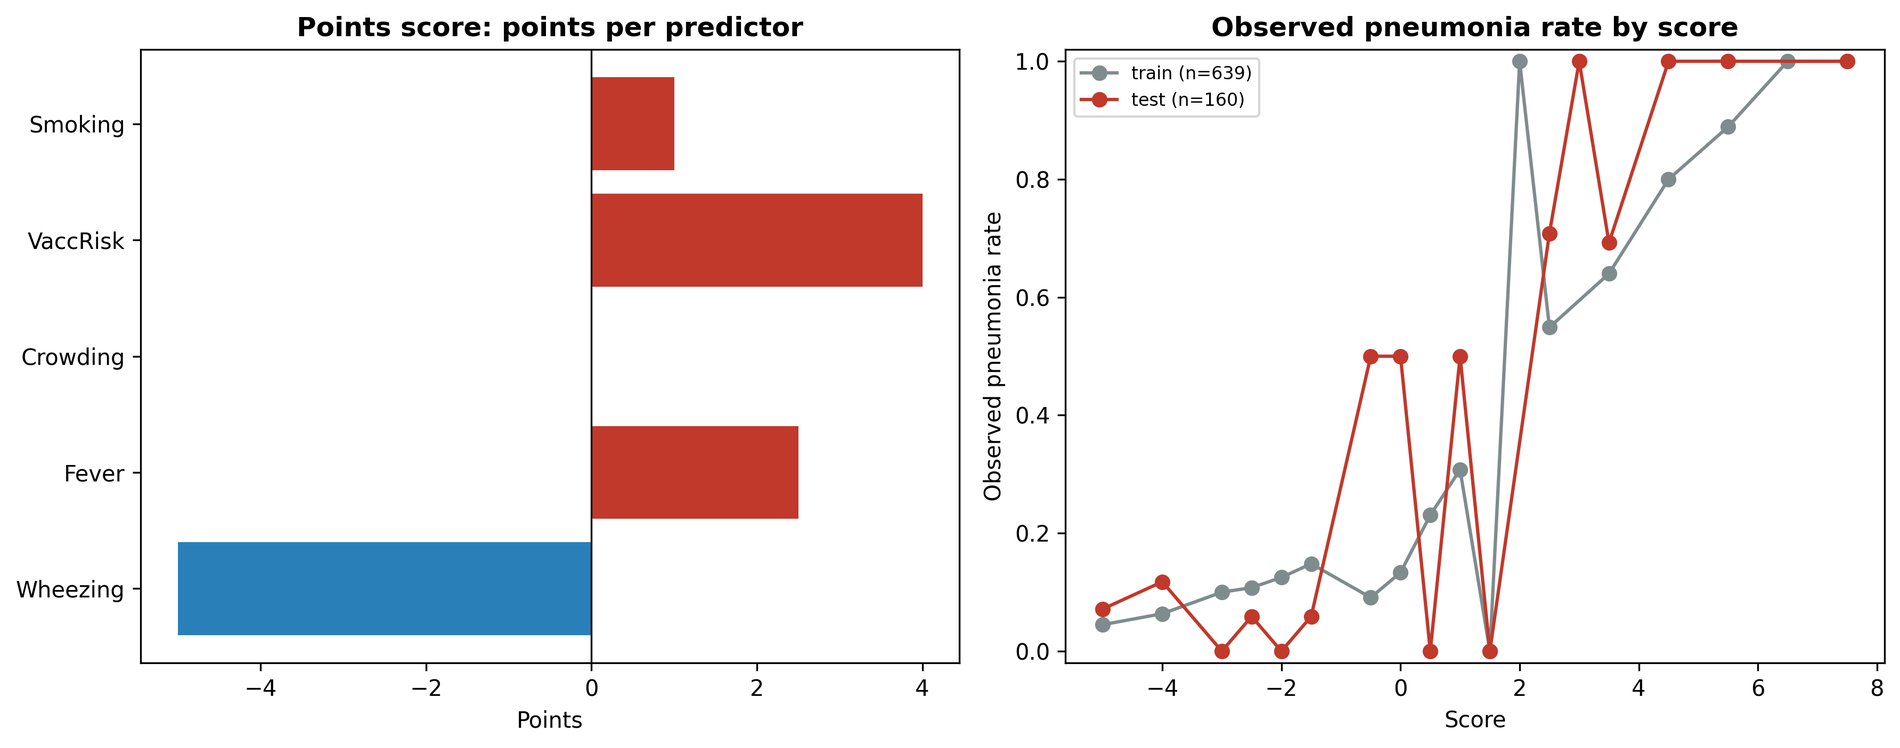
\includegraphics[width=\textwidth]{fig16.png}
\caption{CPSS points per predictor (left) and observed pneumonia rate by score in the training and test sets (right).}
\label{fig:16}
\end{figure*}

\subsection{Fairness and subgroup analysis}
\label{sec:fairr}

Table~\ref{tab:14} and Fig.~\ref{fig:17} show Random Forest performance on the test set by subgroup. AUC ranged from 0.813 (infants $\leq$ 12 months) to 0.952 (not fully vaccinated), and recall at 0.5 from 0.583 (female) to 0.875 (not fully vaccinated). Point estimates were lower in females (AUC 0.815, recall 0.583) than males (0.911, 0.719) and in infants (0.813, 0.619) than older children (0.893, 0.739), but every interval is wide (for example 0.629--0.946 for females, who had only 12 pneumonia cases) and the intervals overlap, so these data neither demonstrate nor exclude a performance difference. The result for children who were not fully vaccinated (n = 21, 8 events) is exploratory only. The analysis shows no collapse of performance in any subgroup, but the subgroup sizes are too small to support a claim of equitable performance, and the lower sensitivity in infants and girls deserves attention in a larger validation.

\begin{table*}[tbp]
\caption{Random Forest performance by subgroup on the test set (AUC with 95\% bootstrap CI; recall at threshold 0.5). $^{\dagger}$ Fewer than 10 positive cases, exploratory.}
\label{tab:14}
\centering
{\scriptsize
\setlength{\tabcolsep}{3.2pt}
\begin{tabular}{>{\raggedright\arraybackslash}p{0.291\textwidth}>{\raggedright\arraybackslash}p{0.070\textwidth}>{\raggedright\arraybackslash}p{0.123\textwidth}>{\raggedright\arraybackslash}p{0.287\textwidth}>{\raggedright\arraybackslash}p{0.144\textwidth}}
\toprule
\textbf{Subgroup} & \textbf{n} & \textbf{Pneumonia (n)} & \textbf{AUC (95\% CI)} & \textbf{Recall} \\
\midrule
Male & 102 & 32 & 0.911 (0.840--0.969) & 0.719 \\
Female & 58 & 12 & 0.815 (0.629--0.946) & 0.583 \\
Infant ($\leq$12 months) & 57 & 21 & 0.813 (0.687--0.918) & 0.619 \\
Older child (>12 months) & 103 & 23 & 0.893 (0.787--0.976) & 0.739 \\
Fully vaccinated & 139 & 36 & 0.872 (0.795--0.937) & 0.639 \\
Not fully vaccinated $^{\dagger}$ & 21 & 8 & 0.952 (0.837--1.000) & 0.875 \\
\bottomrule
\end{tabular}}
\end{table*}

\begin{figure*}[tbp]
\centering
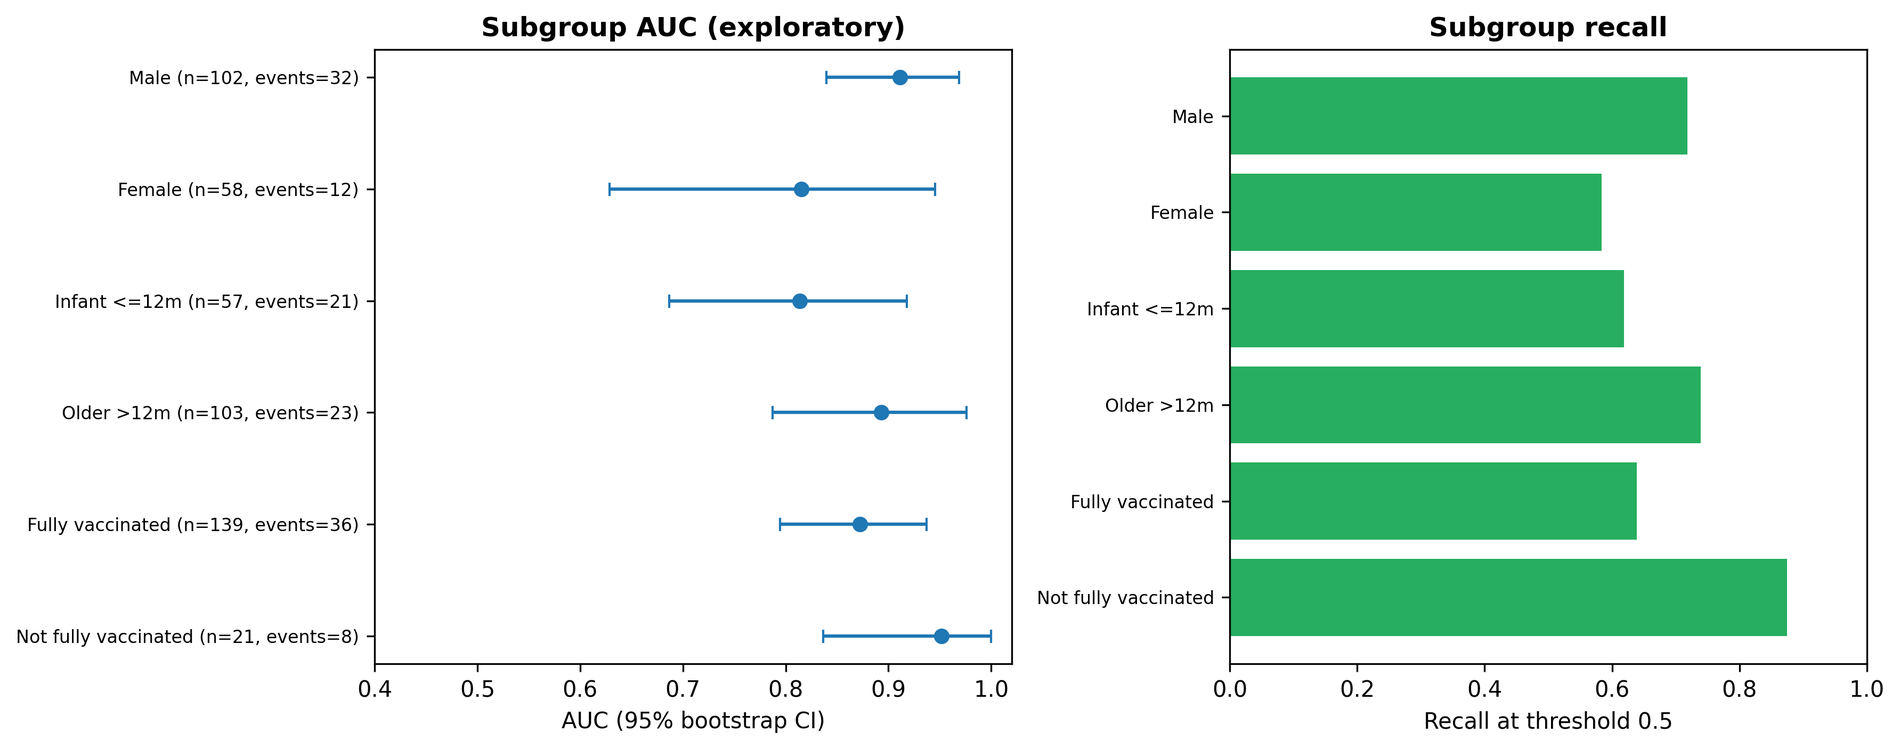
\includegraphics[width=\textwidth]{fig17.png}
\caption{Subgroup AUC with 95\% bootstrap CI (left) and recall at threshold 0.5 (right) for the selected Random Forest model.}
\label{fig:17}
\end{figure*}

\subsection{Sensitivity analysis}

Across ten random train--test splits, Random Forest achieved a mean test AUC of 0.887 (SD 0.021, range 0.856--0.925) and XGBoost 0.883 (SD 0.024, range 0.851--0.928) (Fig.~\ref{fig:18}, Table~\ref{tab:15}). The split-to-split spread (about $\pm$0.02 AUC) is larger than the differences among the leading models, a further reason not to rank them on a single split. As noted in Methods, the hyperparameters were tuned on the seed-42 training set, so values for other seeds are mildly optimistic.

\begin{figure}[tbp]
\centering
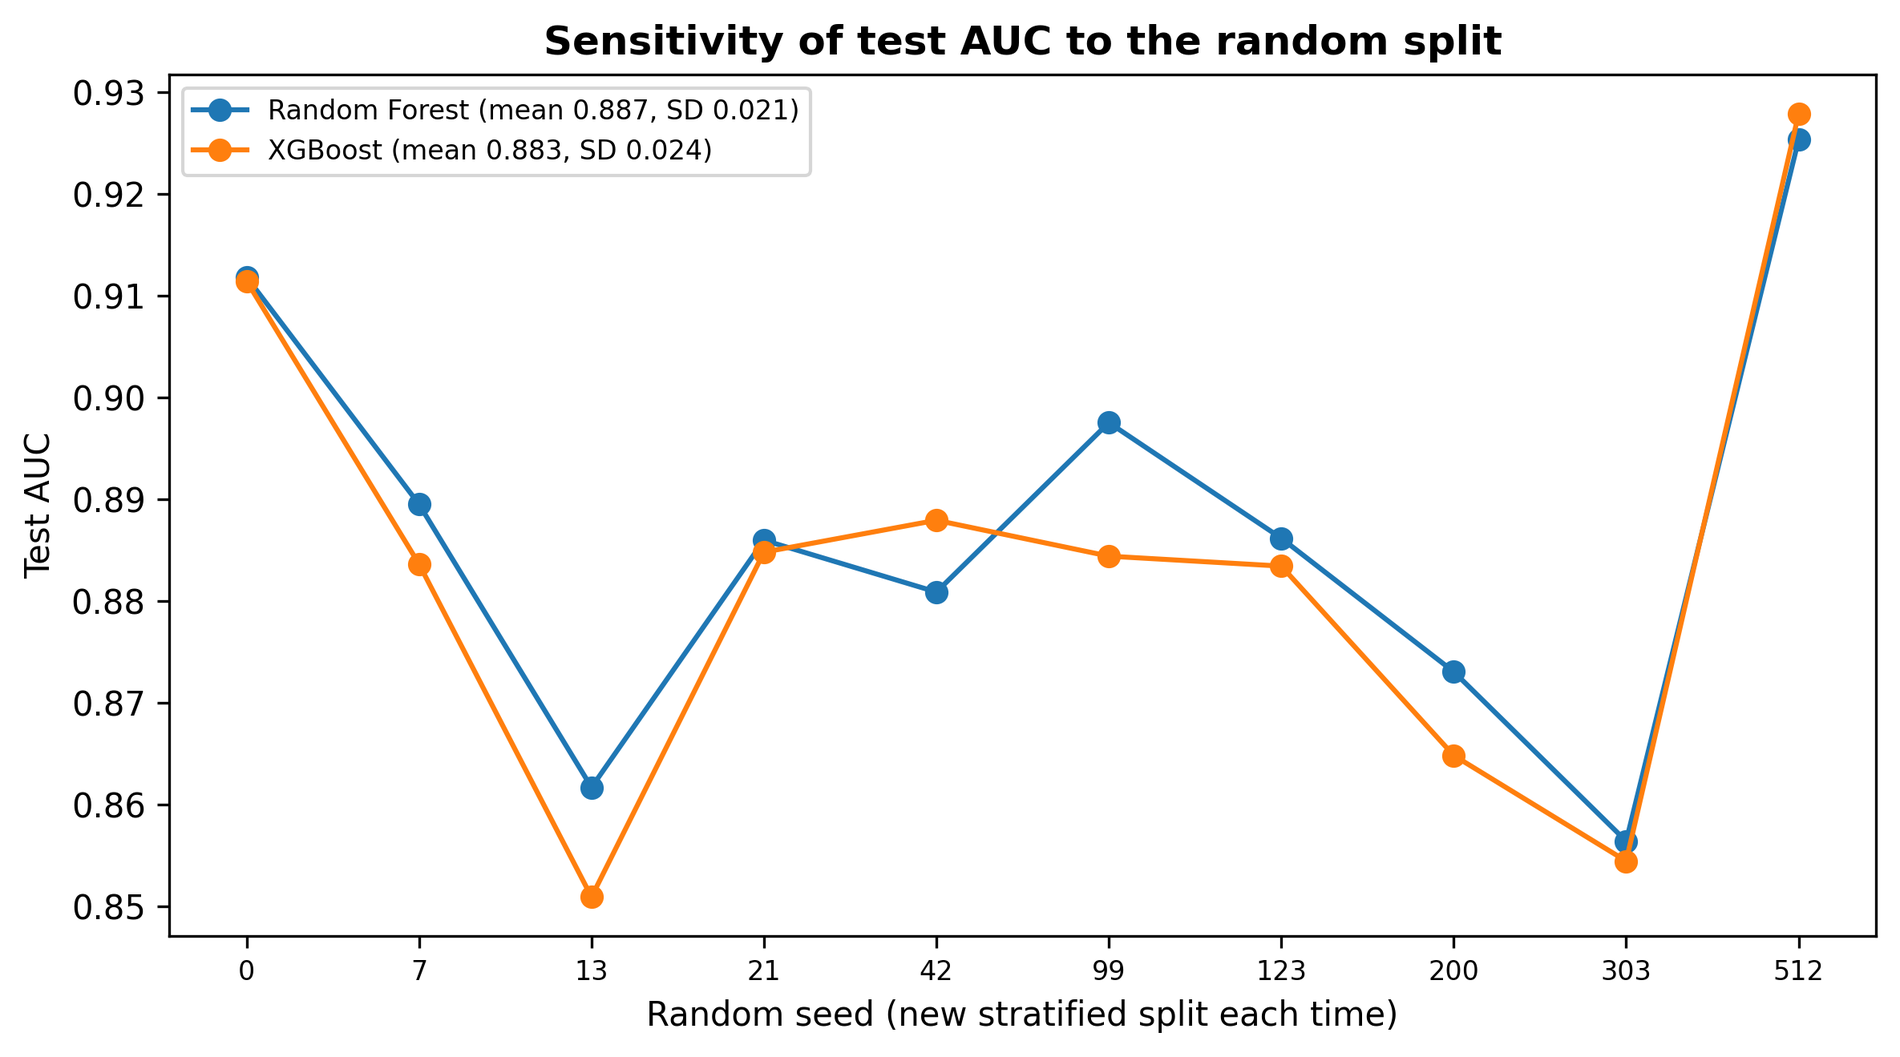
\includegraphics[width=\columnwidth]{fig18.png}
\caption{Test AUC of the tuned Random Forest and XGBoost across ten random stratified splits (hyperparameters not re-tuned).}
\label{fig:18}
\end{figure}

\begin{table}[tbp]
\caption{Test AUC by random seed (new stratified 80/20 split per seed).}
\label{tab:15}
\centering
{\footnotesize
\setlength{\tabcolsep}{3.2pt}
\begin{tabular}{>{\raggedright\arraybackslash}p{0.287\columnwidth}>{\raggedright\arraybackslash}p{0.306\columnwidth}>{\raggedright\arraybackslash}p{0.306\columnwidth}}
\toprule
\textbf{Seed} & \textbf{Random Forest} & \textbf{XGBoost} \\
\midrule
0 & 0.912 & 0.911 \\
7 & 0.889 & 0.884 \\
13 & 0.862 & 0.851 \\
21 & 0.886 & 0.885 \\
42 & 0.881 & 0.888 \\
99 & 0.898 & 0.884 \\
123 & 0.886 & 0.883 \\
200 & 0.873 & 0.865 \\
303 & 0.856 & 0.854 \\
512 & 0.925 & 0.928 \\
Mean (SD) & 0.887 (0.021) & 0.883 (0.024) \\
\bottomrule
\end{tabular}}
\end{table}

\section{Discussion}

\subsection{Interpretation of main results}
\label{sec:interp}

In this single-centre hospital cohort, tree ensembles discriminated a pneumonia diagnosis well, and the four leading models were statistically indistinguishable, so the choice of Random Forest rests on its nested CV-AUC rather than on demonstrated superiority. Discrimination came almost entirely from clinical variables (wheezing, temperature, procalcitonin and CRP). Socio-environmental variables alone added no discrimination, so the hypothesis that crowding and passive smoking improve prediction was not supported, whereas vaccination status showed a clear community-level gradient. Wheezing was inversely related to the pneumonia label because the comparison group consists of other respiratory diagnoses such as bronchiolitis and asthma. Probabilities from SMOTE-trained models over-predict risk and need recalibration before use.

Regarding fairness, subgroup AUCs by sex, age group and vaccination status ranged from 0.813 to 0.952 with wide confidence intervals, and some subgroups had fewer than 10 events; equal performance across groups therefore cannot be claimed or excluded with this sample (Section~\ref{sec:fairr}). The 22-predictor CHW model and the five-item points score kept most of the discrimination (test AUC 0.854 and 0.847) without laboratory, radiographic or examination inputs, which is the finding most relevant to low-resource screening, but it still requires testing in community populations.

\subsection{Comparison with existing literature}
\label{sec:lit}

Table~\ref{tab:16} situates CAEPPF against comparable published studies. The test AUC of the selected model (0.881) is close to that of Serin et al. (0.87) and slightly below Demsash et al. (0.91), which used a different population, a larger dataset and nutritional variables. These figures are not directly comparable because outcomes, populations and validation designs differ. This study differs from earlier structured-data work mainly in the breadth of its validation (ablation, nested cross-validation, calibration, decision curves, statistical tests, subgroup and sensitivity analyses) and in its explicit report of null and negative findings for the socio-environmental variables, rather than in discrimination.

\begin{table*}[tbp]
\caption{Comparison with existing ML studies on pediatric pneumonia.}
\label{tab:16}
\centering
{\scriptsize
\setlength{\tabcolsep}{3.2pt}
\begin{tabular}{>{\raggedright\arraybackslash}p{0.165\textwidth}>{\raggedright\arraybackslash}p{0.144\textwidth}>{\raggedright\arraybackslash}p{0.154\textwidth}>{\raggedright\arraybackslash}p{0.165\textwidth}>{\raggedright\arraybackslash}p{0.287\textwidth}}
\toprule
\textbf{Study} & \textbf{Best model} & \textbf{Dataset} & \textbf{Reported performance} & \textbf{Distinction} \\
\midrule
Demsash et al. \cite{r7} & XGBoost & Ethiopian DHS & AUC 0.91 & Nutritional and demographic variables; no ablation, calibration, or subgroup analysis \\
Serin et al. \cite{r4} & Random forest & Turkey, hospital & AUC 0.87 & Severity escalation; no socio-environmental index, calibration or decision curves \\
Salamon \& Ksiazek \cite{r11} & Capsule network & Chest X-ray & Accuracy 97.2\% & Imaging diagnosis; requires radiography \\
Liang \& Zheng \cite{r12} & Deep residual network & Chest X-ray & Accuracy 96.7\% & Transfer learning; requires radiography \\
This study & Random forest (tuned) & Morocco, hospital (n = 799) & Test AUC 0.881 (0.809--0.938); nested CV-AUC 0.883 & Ablation, nested CV, DeLong/McNemar, calibration, DCA, SHAP, subgroup and sensitivity analyses, community-level model \\
\bottomrule
\end{tabular}}
\end{table*}

\subsection{Limitations}
\label{sec:lim}

\begin{itemize}[leftmargin=1.2em,itemsep=2pt,topsep=3pt]
\item \textbf{External generalizability:} All data come from a single tertiary center in Rabat, Morocco (n = 799). The outcome is a hospital admission diagnosis, so the models discriminate pneumonia from other respiratory admissions and do not estimate community prevalence or screening performance among all febrile children. Multi-site external validation is the highest priority.
\item \textbf{Small test set:} The test set contains 160 children and 44 events, so all test-set intervals are wide, the DeLong and McNemar tests have limited power, and calibration and decision curves are noisy. A single split was used for the primary results; the ten-seed analysis addresses split dependence only partly.
\item \textbf{Untuned comparators:} Only four of eleven models were tuned; the other seven used fixed conventional settings. Their lower performance may partly reflect this, and tuning might narrow the gap. Class weighting was not compared with SMOTE.
\item \textbf{Probability calibration:} SMOTE inflated predicted risks. Recalibration helped only modestly, and probabilities should not be interpreted as absolute risks without local recalibration.
\item \textbf{Predictor definitions:} The chest X-ray finding is close to the diagnostic reference standard and is not available in community settings (it is excluded from the community-level model). The persons-per-room cut-off in the CPSS and the list of CHW-collectable predictors are assumptions that were not tuned or validated with CHWs.
\item \textbf{CERS weight derivation:} CERS weights were estimated on the same training data used for model development, and rest on very few unvaccinated children (n = 7 overall). Prospective validation is required.
\item \textbf{Passive smoking measurement:} Binary self-report captures presence but not intensity or duration, limiting discriminatory power.
\item \textbf{Interpretability model:} SHAP explanations describe XGBoost, not the selected Random Forest. Feature importance for Random Forest is impurity-based and biased toward continuous predictors.
\item \textbf{Subgroup analyses:} Subgroups, notably females (12 events) and not fully vaccinated children (n = 21, 8 events), are too small for reliable inference; no formal heterogeneity test was performed.
\item \textbf{Temporal validation and prospective use:} Train--test splits are stratified but random, not time-ordered, and the CPSS has not been prospectively evaluated with community health workers.
\item \textbf{Sample size:} With 799 patients and 218 positive cases, the dataset is suitable for exploratory ML research but at the lower end for confident subgroup analysis and calibration assessment.
\end{itemize}

\subsection{Intended use and implementation considerations}
\label{sec:use}

\textit{Input data.} The pipeline imputes a missing predictor with the training median, so predictions can be produced when a value is missing, but each imputed value removes information; the share of missing values was small in this cohort (at most 7.7\% for any variable, Section~\ref{sec:incl}) and should be monitored in any new setting. Records without a critical variable (CRP, age, respiratory rate or household size) should not be scored. Laboratory and radiographic inputs are not available to CHWs, which is why the 22-predictor CHW model and the five-item score were developed.

\textit{Users and expertise.} The full model needs a clinician and laboratory results. The CHW model and CPSS need training in recording symptoms, vaccination status and household information, and a score computed by hand should be checked against the software version. Outputs are intended as decision support for triage and referral, not as a diagnosis.

\textit{Next steps.} Before any use, the models need external validation in community and primary-care populations (including children without a respiratory diagnosis), recalibration to local prevalence, assessment of fairness in larger subgroups, and a prospective impact study. Applicability beyond this Moroccan hospital cohort is not established.

\section{Conclusion}
\label{sec:conc}

This paper presented CAEPPF, a transparent and reproducible comparison of eleven classifiers for pediatric pneumonia diagnosis in a Moroccan hospital cohort, with full documentation of the algorithms, their settings, the tuning procedure and the selection criterion. Random Forest was selected by nested cross-validation (CV-AUC 0.883; test AUC 0.881), but the four leading models were statistically indistinguishable, so the choice among them should rest on calibration, interpretability and deployment context. Probabilities from SMOTE-trained models over-predicted risk and need recalibration before use as absolute risks.

The ablation did not support the earlier hypothesis that socio-environmental variables add discriminative information to clinical predictors: all 28 predictors improved CV-AUC by 0.011 over the clinical baseline, but socio-environmental variables alone did not. Vaccination status showed the clearest community-level association with pneumonia, while crowding and passive smoking contributed little, and the data-derived CERS discriminated near chance. Wheezing was the dominant and inversely related predictor, reflecting the comparison group. A community-level model using 22 predictors retained a test AUC of 0.854 and a five-item points score reached 0.847, which together indicate that useful risk stratification may be achievable without laboratory infrastructure. These findings are from one hospital and a small test set; multi-site external validation, prospective evaluation of the score with community health workers, and threshold optimization on calibrated probabilities are the necessary next steps before any deployment.

\section*{CRediT authorship contribution statement}

\textbf{Md Artad Chowdhury:} Conceptualization, Investigation, Data curation, Resources, Writing -- original draft. \textbf{Bishal Paul:} Methodology, Software, Formal analysis, Validation, Visualization, Writing -- original draft, Writing -- review \& editing, Supervision, Project administration. \textbf{Md. Asif Mredha:} Formal analysis, Validation, Visualization, Writing -- review \& editing. \textbf{Shafiul Alam Faysal:} Methodology, Software, Validation, Writing -- review \& editing.

\section*{Declaration of competing interest}

The authors declare that they have no known competing financial interests or personal relationships that could have appeared to influence the work reported in this paper.

\section*{Acknowledgments}

The authors thank Tligui, H., Hattoufi, K., Jroundi, I., Mahraoui, C., and Bassat, Q. for compiling and publicly sharing the pediatric respiratory infection dataset used in this study via Mendeley Data (DOI: 10.17632/2d9dvnycjw.1) under a CC BY 4.0 license.

\begin{table*}[tbp]
\caption{TRIPOD+AI checklist \cite{r34}: location of each reporting item in this paper (all items apply to this development and internal-validation study unless marked not applicable or not available).}
\label{tab:tripod}
\centering
{\footnotesize
\begin{tabular}{>{\raggedright\arraybackslash}p{3.6cm}>{\raggedright\arraybackslash}p{1.4cm}>{\raggedright\arraybackslash}p{9cm}}
\toprule
Section/topic & Item & Reported in \\
\midrule
Title & 1 & Title page \\
Abstract & 2 & Abstract (TRIPOD+AI for Abstracts items 1--13) \\
Background & 3a & \S\ref{sec:intro}, \S\ref{sec:litrev} \\
 & 3b & \S\ref{sec:tpop} \\
 & 3c & \S\ref{sec:ineq} \\
Objectives & 4 & \S\ref{sec:obj} \\
Data & 5a & \S\ref{sec:data}, \S\ref{sec:setting} \\
 & 5b & \S\ref{sec:setting} (dates to be inserted) \\
Participants & 6a & \S\ref{sec:setting} \\
 & 6b & \S\ref{sec:setting}, \S\ref{sec:incl} \\
 & 6c & \S\ref{sec:setting} \\
Data preparation & 7 & \S\ref{sec:incl}, \S\ref{sec:prep} \\
Outcome & 8a & \S\ref{sec:data} \\
 & 8b & Not available (public data) \\
 & 8c & Not applicable (retrospective) \\
Predictors & 9a & \S\ref{sec:feat}, \S\ref{sec:fsel} \\
 & 9b & \S\ref{sec:feat} \\
 & 9c & Not available (public data) \\
Sample size & 10 & \S\ref{sec:ss} \\
Missing data & 11 & \S\ref{sec:incl} \\
Analytical methods & 12a & \S\ref{sec:part} \\
 & 12b & \S\ref{sec:prep} \\
 & 12c & \S\ref{sec:alg}, \S\ref{sec:hyp}, \S\ref{sec:sel} \\
 & 12d & \S\ref{sec:trev} \\
 & 12e & \S\ref{sec:perf}, \S\ref{sec:stat}, \S\ref{sec:calm}, \S\ref{sec:dcam} \\
 & 12f & \S\ref{sec:calm} \\
 & 12g & \S\ref{sec:output} \\
Class imbalance & 13 & \S\ref{sec:prep} \\
Fairness & 14 & \S\ref{sec:fairm}, \S\ref{sec:fairr} \\
Model output & 15 & \S\ref{sec:output} \\
Training vs evaluation & 16 & \S\ref{sec:trev} \\
Ethical approval & 17 & \S\ref{sec:eth} \\
Open science & 18a--f & \S\ref{sec:open} (funding, conflicts, protocol, registration, data and code sharing); Declaration of competing interest \\
Patient and public involvement & 19 & \S\ref{sec:open} \\
Participants (results) & 20a & \S\ref{sec:incl}, \S\ref{sec:cohort} \\
 & 20b & \S\ref{sec:cohort}; Table~\ref{tab:1} \\
 & 20c & Not applicable (no external evaluation data) \\
Model development & 21 & \S\ref{sec:part}, \S\ref{sec:ss} \\
Model specification & 22 & \S\ref{sec:output}; S1 File \\
Model performance & 23a & \S\ref{sec:mperf}, \S\ref{sec:fairr} \\
 & 23b & Not applicable (single centre) \\
Model updating & 24 & \S\ref{sec:calr} \\
Interpretation & 25 & \S\ref{sec:interp}, \S\ref{sec:lit}, \S\ref{sec:conc} \\
Limitations & 26 & \S\ref{sec:lim} \\
Usability & 27a--b & \S\ref{sec:use} \\
 & 27c & \S\ref{sec:use}, \S\ref{sec:conc} \\
\bottomrule
\end{tabular}}
\end{table*}

\begin{thebibliography}{34}
\bibitem{r1} M S, Vaithilingan S. Childhood pneumonia in low- and middle-income countries: A systematic review of prevalence, risk factors, and healthcare-seeking behaviors. Cureus. 2024;16(4): e57636. doi:10.7759/cureus.57636.
\bibitem{r2} Kenganal R, Basavaraj, Mavinahalli A, Sanikam H. Clinical and socio-demographic profile of pneumonia in children. Panacea J Med Sci. 2024; 14:204--209.
\bibitem{r3} Kamruzzaman M, Rahman MA, Hasan MJ, Islam MS. Risk factors of pneumonia in children: A study in Bangladesh. Am J Pediatr. 2025;11(1):7--13.
\bibitem{r4} Serin O, Gunay S, Aksoy F, Simsek D. Predicting escalation of care for childhood pneumonia using machine learning. JMIRx Med. 2025;6: e57719.
\bibitem{r5} Marangu D, Zar HJ. Childhood pneumonia in low- and middle-income countries: An update. Paediatr Respir Rev. 2019; 32:3--9.
\bibitem{r6} Lu Y. Determinants of childhood pneumonia: A retrospective analysis. Front Med (Lausanne). 2025;12.
\bibitem{r7} Demsash AW, Bekele MM, Walle AD, Amsalu ET, Chereka AA, Tarekegn BT, et al. Data-driven machine learning algorithm for pneumonia prediction among children in Ethiopia. BMC Infect Dis. 2025;25(1):647.
\bibitem{r8} Howie SRC, Schellenberg J, Chimah O, Ideh RC, Ebruke BE, Oluwalana C, et al. Childhood pneumonia and crowding, bed-sharing and nutrition: A case-control study from The Gambia. Int J Tuberc Lung Dis. 2016;20(10):1405--1415.
\bibitem{r9} da Fonseca Lima EJ, Mello MJG, Albuquerque MFPM, Lopes MIL, Serra GHC, Lima DEP, et al. Risk factors for community-acquired pneumonia in children under five years of age in the post-pneumococcal conjugate vaccine era in Brazil: A case control study. BMC Pediatr. 2016;16(1):157.
\bibitem{r10} Nyuydzedze SS, Kamgno J, Nkwescheu AS. Predictors of community acquired pneumonia in children in Cameroon. J Public Health Epidemiol. 2024;16(3).
\bibitem{r11} Salamon S, Ksiazek W. Capsule neural networks for pediatric pneumonia detection from chest x-ray. J Clin Med. 2025;14(20).
\bibitem{r12} Liang G, Zheng L. A transfer learning method with deep residual network for pediatric pneumonia diagnosis. Comput Methods Programs Biomed. 2020; 187:104964.
\bibitem{r13} Barday MM, Slogrove AL, Engelbrecht AL. Risk factors associated with severity of pneumonia. J Pan Afr Thorac Soc. 2022;3(3).
\bibitem{r14} Osman RI, Mohammed SH, Ahmed AE. Magnitude and associated factors of pneumonia among under-five children in Ethiopia. BMC Pediatr. 2025;25(1).
\bibitem{r15} Tligui H, Hattoufi K, Jroundi I, Mahraoui C, Bassat Q. Pediatric respiratory infections: Epidemiological and etiological data from a cohort of 801 Moroccan children [data set]. Mendeley Data, V1; 2024. doi:10.17632/2d9dvnycjw.1.
\bibitem{r16} DeLong ER, DeLong DM, Clarke-Pearson DL. Comparing the areas under two or more correlated receiver operating characteristic curves: A nonparametric approach. Biometrics. 1988;44(3):837--845.
\bibitem{r17} Chawla NV, Bowyer KW, Hall LO, Kegelmeyer WP. SMOTE: synthetic minority over-sampling technique. J Artif Intell Res. 2002;16:321--357.
\bibitem{r18} Breiman L. Random forests. Mach Learn. 2001;45(1):5--32.
\bibitem{r19} Chen T, Guestrin C. XGBoost: a scalable tree boosting system. Proceedings of the 22nd ACM SIGKDD International Conference on Knowledge Discovery and Data Mining. 2016:785--794.
\bibitem{r20} Ke G, Meng Q, Finley T, Wang T, Chen W, Ma W, et al. LightGBM: a highly efficient gradient boosting decision tree. Adv Neural Inf Process Syst. 2017;30:3146--3154.
\bibitem{r21} Bergstra J, Bengio Y. Random search for hyper-parameter optimization. J Mach Learn Res. 2012;13:281--305.
\bibitem{r22} Cawley GC, Talbot NLC. On over-fitting in model selection and subsequent selection bias in performance evaluation. J Mach Learn Res. 2010;11:2079--2107.
\bibitem{r23} Pedregosa F, Varoquaux G, Gramfort A, Michel V, Thirion B, Grisel O, et al. Scikit-learn: machine learning in Python. J Mach Learn Res. 2011;12:2825--2830.
\bibitem{r24} Lundberg SM, Lee SI. A unified approach to interpreting model predictions. Adv Neural Inf Process Syst. 2017;30:4765--4774.
\bibitem{r25} Grinsztajn L, Oyallon E, Varoquaux G. Why do tree-based models still outperform deep learning on typical tabular data? Adv Neural Inf Process Syst. 2022;35:507--520.
\bibitem{r26} Sun X, Xu W. Fast implementation of DeLong’s algorithm for comparing the areas under correlated receiver operating characteristic curves. IEEE Signal Process Lett. 2014;21(11):1389--1393.
\bibitem{r27} Vickers AJ, Elkin EB. Decision curve analysis: a novel method for evaluating prediction models. Med Decis Making. 2006;26(6):565--574.
\bibitem{r28} Van Calster B, McLernon DJ, van Smeden M, Wynants L, Steyerberg EW. Calibration: the Achilles heel of predictive analytics. BMC Med. 2019;17:230.
\bibitem{r29} Platt J. Probabilistic outputs for support vector machines and comparisons to regularized likelihood methods. In: Smola AJ, Bartlett P, Sch\"olkopf B, Schuurmans D, editors. Advances in Large Margin Classifiers. Cambridge, MA: MIT Press; 1999. p. 61--74.
\bibitem{r30} van den Goorbergh R, van Smeden M, Timmerman D, Van Calster B. The harm of class imbalance corrections for risk prediction models: illustration and simulation using logistic regression. J Am Med Inform Assoc. 2022;29(9):1525--1534.
\bibitem{r31} Freund Y, Schapire RE. A decision-theoretic generalization of on-line learning and an application to boosting. J Comput Syst Sci. 1997;55(1):119--139.
\bibitem{r32} Cortes C, Vapnik V. Support-vector networks. Mach Learn. 1995;20(3):273--297.
\bibitem{r33} McNemar Q. Note on the sampling error of the difference between correlated proportions or percentages. Psychometrika. 1947;12(2):153--157.
\bibitem{r34} Collins GS, Moons KGM, Dhiman P, et al. TRIPOD+AI statement: updated guidance for reporting clinical prediction models that use regression or machine learning methods. BMJ. 2024;385:e078378. doi:10.1136/bmj-2023-078378.
\end{thebibliography}

\end{document}
